\documentclass[en,twoside,onehalfspacing,msc]{risethesis}

\usepackage{colortbl}
\usepackage{color}
\usepackage[table]{xcolor}
\usepackage{microtype}
\usepackage{bibentry}
\usepackage{subfigure}
\usepackage{multirow}
\usepackage{rotating}
\usepackage{booktabs}
\usepackage{pdfpages}
\usepackage[labelfont=bf,font=footnotesize,justification=centering]{caption}
\usepackage{lipsum}
\usepackage{sectsty}
\usepackage{listings}
\usepackage[newfloat]{minted}
\usepackage[htt]{hyphenat} % Allow hyphenation inside \texttt

% savenotes env to enable footnote inside tables or figures
\usepackage{footnote} % needs to be after xcolor

%% Change the following pdf author attribute name to your name.
\usepackage[linkcolor=black,
            citecolor=blue, % XXX: final version should be black
            urlcolor=black,
            colorlinks,
            pdfpagelabels,
            breaklinks=true,
            pdftitle={M.Sc. Thesis - Luís Gabriel Lima},
            pdfauthor={Luís Gabriel Lima}]{hyperref}

% Should be imported after hyperref
\usepackage[alf]{abntex2cite}

\captionsetup[table]{position=top,width=.85\textwidth}
\captionsetup[lstlisting]{position=top,width=.85\textwidth}
\captionsetup[figure]{position=bottom,width=.85\textwidth}

%% Chapter and (Sub)Section fonts must be same size as text (12)
\sectionfont{\fontsize{12}{15}\selectfont}
\subsectionfont{\fontsize{12}{15}\selectfont}
\subsubsectionfont{\fontsize{12}{15}\selectfont}

\SetupFloatingEnvironment{listing}{name={\lstlistingname}, fileext=lol}

\setminted[haskell]{linenos=true,frame=lines,framesep=2mm,fontsize=\footnotesize}
\setminted[text]{linenos=true,frame=lines,framesep=2mm,fontsize=\footnotesize}

% import our custom commands

\newcommand{\codeterm}[1]{\texttt{#1}\xspace}

\newcommand{\forkIO}{\codeterm{forkIO}}
\newcommand{\forkOn}{\codeterm{forkOn}}
\newcommand{\forkOS}{\codeterm{forkOS}}


\address{RECIFE}

\universitypt{Universidade Federal de Pernambuco}
\universityen{Federal University of Pernambuco}

\departmentpt{Centro de Informática}
\departmenten{Informatics Center}

\programpt{Pós-graduação em Ciência da Computação}
\programen{Graduate in Computer Science}

\majorfieldpt{Ciência da Computação}
\majorfielden{Computer Science}

\title{Understanding the Energy Behavior of Concurrent Haskell Programs}

\date{2016}

\author{Luís Gabriel Nunes Ferreira Lima}
\adviser{Fernando José Castor de Lima Filho}
\coadviser{João Paulo de Sousa Ferreira Fernandes}

% Macros (defines your own macros here, if needed)
\def\x{\checkmark}

\begin{document}

\frontmatter

\frontpage

\presentationpage

\begin{fichacatalografica}
	\FakeFichaCatalografica % Comment this line when you have the correct file
%     \includepdf{fig_ficha_catalografica.pdf} % Uncomment this
\end{fichacatalografica}

\banca

\begin{dedicatory}
To my parents.
\end{dedicatory}

\acknowledgements
\lipsum[1-4]

\begin{epigraph}[True Detective: After You've Gone]{Rustin Cohle}
Life's barely long enough to get good at one thing.
\linebreak
So be careful what you get good at.
\end{epigraph}

\resumo
Há anos eficiência energética é uma preocupação para designers de hardware e software baixo-nível. Entretanto, a rápida proliferação de dispositivos móveis alimentados por bateria combinado com o crescente movimento global em busca de sustentabilidade tem motivado desenvolvedores e pesquisadores a estudar o impacto energético de softwares de aplicação em execução. Trabalhos recentes tem estudado o efeito de fatores como obsfucação de código, refatorações em linguagem orientadas à objetos e tipos de dados tem em eficiência energética. Este trabalho tenta lançar luz sobre o comportamento energético de programas concorrentes escritos em uma linguagem puramente funcional, Haskell.

Nós conduzimos um estudo empírico para avaliar o desempenho e o comportamento energético de três diferentes abordagens para gerenciamento de threads e três primitivas para controle de concorrência usando nove diferentes benchmarks com um espaço de exploração experimental de mais de 400 configurações. Neste estudo, descobrimos que pequenas mudanças podem fazer uma grande diferença em termos de consumo de energia. Por exemplo, em um dos benchmarks, sob uma configuração específica, escolher uma primitiva de controle de concorrência (MVar) ao invés de outra (TMVar) pode acarretar em uma economia de 60\% em consumo de energia. Percebemos também que nem sempre a relação entre consumo de energia e desempenho é clara. Em alguns cenários analisados, a configuração com melhor desempenho também apresentou o pior consumo de energia.

Para ajudar desenvolvedores a entender melhor essa complexa relação, nós estendemos duas ferramentas de análise de desempenho existentes para coletar e apresentar dados sobre consumo de energia. Adicionalmente, baseado nos resultados do nosso estudo empírico, listamos um conjunto de recomendações para desenvolvedores com boas práticas de como escrever código energeticamente eficiente nesse ambiente.

\begin{keywords}
Eficiência Energética, Consumo de Energia, Haskell, Programação Concorrente, Programação Funcional, Análise de Desempenho
\end{keywords}


\abstract
\lipsum[1-4]

\begin{keywords}
Software Engineering, Software Maintenance and Evolution, Change Request
Management, Automatic Change Request Assignment
\end{keywords}


\listoffigures

\listoftables

\lstlistoflistings

% Acronyms manual: http://linorg.usp.br/CTAN/macros/latex/contrib/acronym/acronym.pdf
\listofacronyms
\begin{acronym}[ACRONYM]
% Change the word ACRONYM above to change the acronym column width.
% The column width is equals to the width of the word that you put.
% Read the manual about acronym package for more examples:
%   http://linorg.usp.br/CTAN/macros/latex/contrib/acronym/acronym.pdf
\acro{csp}[CSP]{Communicating Sequential Processes}
\acro{tm}[TM]{Transactional Memory}
\acro{stm}[STM]{Software Transactional Memory}
\acro{ghc}[GHC]{Glasgow Haskell Compiler}
\acro{rts}[RTS]{GHC runtime system}
\acro{hec}[HEC]{Haskell Execution Context}
\acro{api}[API]{Application Programming Interface}
\end{acronym}


% Summary (tables of contents)
\tableofcontents

\mainmatter

\chapter{Introduction}\label{chp:introduction}

% \begin{quotation}[]{Poul Anderson}
% I have yet to see any problem, however complicated, which, when looked at in the
% right way, did not become still more complicated.
% \end{quotation}

The evolution of technology is unveiling a reality that could hardly be imaginable some decades ago. Nowadays, we can buy a multiprocessor computer with a few gigabytes of memory with the size of a credit card for less than a hundred dollars. The ability to manufacture such small and potent devices is leading to a rapid proliferation of a variety of mobile computing platforms. These devices are part of a diverse ecosystem that includes smartwatches, smartphones, tablets, IoT sensors, and drones. In this sort of device, it is imperative for delivering a good user experience that they stay up and running for as long as possible. So \emph{energy consumption} is a huge concern in this universe as it is closely related to battery lifetime. %% XXX: the conclusion still need some love

This concern, however, goes beyond unwired devices. On the other side of the spectrum, big internet companies are also affected by low energy efficiency. To deliver fast access to its services globally, these companies usually have to maintain a huge server infrastructure to host its products. In this kind of environment, due to its scale, the energy consumption can have a high impact on the maintenance costs. For instance, Facebook is building data centers inside the Arctic Circle in order to improve the system's energy efficiency by reducing the power needed for cooling\footnote{\scriptsize\url{http://www.bloomberg.com/news/articles/2013-10-04/facebooks-new-data-center-in-sweden-puts-the-heat-on-hardware-makers}}. This is just one example of the economic impact driven by the seek for more efficient solutions. It shows that energy efficiency is becoming a key design attribute for building computational systems.

Although it may seem like a recent problem, the energy efficiency of computer systems has been a concern for researchers for a long time. Initially, most of the research focused on the hardware design layer, developing new ways to build electronic components that wasted less energy~\cite{chandrakasan:1992}. This was motivated by the assumption that only hardware dissipates power, not software. However, in a computer system, software plays a fundamental role in deciding how a computational task will be executed on specific hardware. For this reason, software can have a substantial impact on energy consumption.

From a software perspective, the energy efficiency problem can be tackled at different levels of abstraction, ranging from machine code level to user-facing applications. Traditionally, the research in this area has been focused on low-level software. Much progress has been achieved on building energy-efficient solutions for embedded software~\cite{tiwari:1994}, compilers~\cite{hsu:2003}, operating systems~\cite{merkel:2006} and runtime systems~\cite{ribic:2014, farkas:2000}. However, the growing worldwide movement towards sustainability, including sustainability in software~\cite{becker:2015}, have motivated the study of the energy impact of application software in execution.

Recent empirical studies have provided initial evidence that high-level decisions can effectively reduce the energy usage of an application software~\cite{chung:2001,hindle:2012,pinto:2014,trefethen:2013,manotas:2014,sahin:2014}. It is important to note that optimizing software at the application level does not cancel the lower level optimizations. They are complementary solutions. However, it is still not clear which software engineering practices are beneficial for saving energy. A recent study by~\citeonline{pinto:2014b} shows that, although application developers are consistently more interested in understanding how to reduce energy consumption in their software, there is a general lack of information in the community about how it can be achieved.


\section{Problem}
\lipsum[1-2]


\section{Goal}
\lipsum[3-4]


\section{Contributions}
This work sheds light on the energy behavior of Haskell programs. To the best of our knowledge, this is the first attempt to analyze energy efficiency in the context of functional programming languages. Moreover, this work makes the following contributions:

\begin{itemize}
  \item \textbf{A tool for fine-grained energy analysis.} We extend the \acs{ghc} profiler to collect and report fine-grained information about the energy consumption of a Haskell program;
  \item \textbf{A tool for coarse-grained energy analysis.} We extend the Criterion microbenchmarking library to collect, perform and report statistical performance analysis of the energy consumption of Haskell code;
  \item \textbf{An understanding of the energy behavior of concurrent Haskell programs.} We conduct an extensive experimental space exploration illuminating the relationship between the choices and settings of Haskell's concurrent programming constructs, and performance and energy consumption over real-world Haskell benchmarks;
  \item \textbf{A list of guidelines on how to write energy-efficient software in Haskell.} We provide some recommendations for helping software developers to write energy-efficient Haskell programs.
\end{itemize}

\section{Outline}
The remainder of this work is structured as follows.

\textbf{\chapref{chp:background}} reviews essential concepts used throughout this work. First, we briefly introduce the Haskell programming language. We show through a series of code samples some important and distinct features of the language. Second, we present an overview of the fundamentals of concurrent programming. Finally, we present how Haskell approaches concurrent programming. We show which abstractions the language provides for both creating new threads of execution and sharing data among these threads. We also present an overview of how the Haskell's runtime system handles threading on multiprocessors.

In \textbf{\chapref{chp:tools}}, we show how to measure the energy consumption of Haskell programs. First, we explain what is \acs{rapl} and how it can be used to collect energy data. Then, we present in details two performance analysis tools of the Haskell ecosystem that we extended to also work with the energy consumption metric.

\textbf{\chapref{chp:study}} shows how different concurrent constructs impact energy consumption. We present an empirical study that we conducted considering three distinct thread management constructs and primitives for sharing data. Through an extensive experimental space exploration over real-world Haskell benchmarks, we produce a list of findings about the energy behaviors of concurrent Haskell programs, which are not always obvious.

In \textbf{\chapref{chp:guide}}, we present a list of recommendations for Haskell developers on how to write energy-efficient software. These recommendations are based on the results of our empirical study.

Finally, \textbf{\chapref{chp:related}} discusses previous research related to this work and \textbf{\chapref{chp:conclusion}} present our concluding remarks and discuss where this work might lead.

\chapter{Background}
In this chapter we review and introduce some essential concepts used in this work. First, we give a short introduction on the Haskell Programming Language. Later we describe briefly the fundamentals of concurrency and the approaches for concurrent programming in Haskell. Finally, we discuss important concepts of software energy consumption.

\section{Haskell}
Haskell is a \emph{purely functional} programming language. By functional, we mean that functions are the building blocks of programs written in Haskell. By pure, we mean that no side-effect happens when evaluating a function. While in imperative programming languages, a program is expressed as a sequence of instructions that mutates data, a program in functional programming languages is expressed as a composition of expressions where all state is controlled by passing arguments to function calls and returning values from them. This property is called \emph{referential transparency}. It guarantees that in a given execution context, a function executed with a given argument will always produce the same result. This property makes it easier to reason about programming as it enforces that a program's behavior cannot depend on history.

Haskell is also a \emph{lazy} programming language. Lazy refers to a non-strict evaluation strategy also known as \emph{call-by-need}. This strategy delays the evaluation of an expression until its value is needed. It avoids repeated evaluations which can lead to performance improvements. This strategy also makes it possible to construct potentially infinite data structures.

\emph{Recursion} is the norm in a purely functional programming language as regular iterative loops require state mutation. To make it easier to express recursive functions, Haskell also has \emph{pattern matching}. In Code \ref{code:fact}, we can see an example of a recursive function using pattern matching. Line 1 is the base case, when the \texttt{factorial} receives zero as parameter, and Line 2 is the general case.

\begin{listing}
  \begin{minted}{haskell}
factorial :: Int -> Int
factorial 0 = 1
factorial x = x * factorial (x - 1)
  \end{minted}
  \caption{A recursive factorial function}
  \label{code:fact}
\end{listing}

Another characteristic of Haskell is that functions are values. It means that a function can receive other functions as argument, and also can be the result of a function evaluation. This feature is known as \emph{high-order functions}. It enables very popular functional patterns such as \texttt{map}, \texttt{filter} and \texttt{reduce}.

Functions in Haskell can also be \emph{polymorphic}, which means that a function can be generalized to work with multiple types instead of a single one. Other programming languages have similar features such as \emph{generics} in Java and \emph{templates} in C++. Code \ref{code:poly} shows an example of a polymorphic function that can reverse a list of any type. In this example, \texttt{t} is a \emph{parametric type}~\citep{cardelli:1985} used to bind the input type to the output type of \texttt{reverse}.

\begin{listing}
  \begin{minted}{haskell}
reverse :: [t] -> [t]
reverse l = rev l []
  where
    rev []     a = a
    rev (x:xs) a = rev xs (x:a)
  \end{minted}
  \caption{A polymorphic function to reverse a list}
  \label{code:poly}
\end{listing}

In Haskell, a developer can also extend the built-in primitive types by defining new \emph{abstract data types}. Code \ref{code:tree} shows an example defining the \texttt{Tree} data type and the function \texttt{depth} to calculate the depth of the tree. As this example shows, the parametric polymorphism also works for abstract data types. Here, \texttt{Tree} have two constructors \texttt{Node} and \texttt{Empty}, where the first one holds three elements: the value of the node, the, left and right sub-trees. Pattern matching can be used to walk through a \texttt{Tree} as shown in Lines 5 and 6.

\begin{listing}
  \begin{minted}{haskell}
data Tree t = Node t (Tree t) (Tree t)
            | Empty

depth :: Tree t -> Int
depth Empty        = 0
depth (Node _ l r) = 1 + max (depth l) (depth r)
  \end{minted}
  \caption{A data type for binary tree and a function to calculate its depth}
  \label{code:tree}
\end{listing}

There is also a concept called \emph{typeclasses} that enhances the definition of new types in Haskell. A typeclass is similar to an interface. It defines a set of functions that can be applied to a particular type. Typeclasses were designed as a way for implementing ad hoc polymorphism in Haskell. Code \ref{code:tree-eq} shows an example of instantiation of the \texttt{Eq} typeclass for the \texttt{Tree} type we defined earlier. It states that a \texttt{Tree} is comparable for equality if its contained type is also comparable for equality.

\begin{listing}
  \begin{minted}{haskell}
instance Eq a => Eq (Tree a) where
  (==) Empty Empty = True
  (==) Empty (Node _ _ _) = False
  (==) (Node _ _ _) Empty = False
  (==) (Node x xl xr) (Node y yl yr) = (x == y) && (xl == yl) && (xr == yr)
  \end{minted}
  \caption{Definition of an Eq typeclass instance for the Tree data type}
  \label{code:tree-eq}
\end{listing}

The \texttt{Monad} typeclass is particularly important for Haskell because it allow developers to emulate mutable behavior and side-effects in a purely functional manner. Its definition can be seen in Code \ref{code:monad}. The most important functions of this interface are \texttt{(>==)}, also known as \emph{bind}, and \texttt{return}, also called \emph{unit}. The first one binds the contained value of the monad \texttt{m} to the argument of its argument function, and the second wraps a value in the monad \texttt{m} and returns it. It is a common idiom to call a \emph{monad} any type that is an instance of class \texttt{Monad}.

\begin{listing}
  \begin{minted}{haskell}
class Monad m where
  (>>=)  :: m a -> (a -> m b) -> m b
  (>>)   :: m a -> m b -> m b
  return :: a -> m a
  fail   :: String -> m a
  \end{minted}
  \caption{Definition of type class Monad}
  \label{code:monad}
\end{listing}

Two monads are particularly important for this work: \texttt{IO} and \texttt{STM}. The first one defines an environment to execute input/output operations. The second defines an environment for Software Transactional Memory, which is presented in Section \ref{sec:haskell-conc}. In Code \ref{code:io}, we have an example of the use of \texttt{Monad} operators to perform I/O. For instance, the functions \texttt{putStrLn} and \texttt{getLine} from the module \texttt{System.IO} prints and reads a \texttt{String} from the standard I/O, respectively. The result type of \texttt{main} is \texttt{IO ()}, where \texttt{()} is an empty tuple value. It represents that no value is returned, analogous to the type \texttt{void} on imperative languages.

\begin{listing}
  \begin{minted}{haskell}
main :: IO ()
main = putStrLn "What is your name?" >> getLine
       >>= \name -> putStrLn ("Hey " ++ name ++ ", you rock!")
  \end{minted}
  \caption{An example using the Monad operators for the IO type}
  \label{code:io}
\end{listing}

\begin{listing}
  \begin{minted}{haskell}
main :: IO ()
main = do
  putStrLn "What is your name?"
  name <- getLine
  putStrLn ("Hey " ++ name ++ ", you rock!")
  \end{minted}
  \caption{An example using the do notation}
  \label{code:io-do}
\end{listing}

Finally, there is a notation in Haskell that makes it easier to express operation within a monad, the \emph{do-notation}. Code \ref{code:io-do} shows the same example of Code \ref{code:io} rewritten using do-notation. Using \texttt{do}, a series of monadic function calls is sequenced as if in an imperative program. It works mainly as syntactic sugar for \texttt{(>==)} and \texttt{(>>)} calls, binding variables that later become argument of other functions and mainly sequentially composing the calls.


\section{Concurrency}
Concurrency and concurrent programming are on the rise nowadays due to the proliferation of multicore processors. However, these concepts are present in computer science since the early 1970s with the introduction of \emph{time-sharing}~\citep{lea:2006}. This model enables, for example, multi-tasking, which allows users to do several things at the same time in a computer such as browsing the internet, playing music and writing a document. To make this possible, the operating system scheduler has to share the processor time between all other processes that want to use this resource. By doing so, the user feels like the programs are executing at the same time although the processor is actually executing each program in a different time slice.

Concurrency is also usually associated (sometimes indistinctly) to parallelism. Although they are similar concepts, they are not the same. Concurrency consists in interleaving the execution of multiple processes through time-sharing techniques as a way to simulate simultaneity. On the other hand, parallelism is concerned with improving a program's performance. This improvement is achieved by executing several instructions in parallel, which require a multicore processor. Depending on the number of cores available, the execution of a program can be literally parallel, entirely time-shared, or a combination of both.

In concurrent programming, a process is a self-contained execution environment that holds all the information needed to run a program. Creating a new process requires a lot of computational resources such as memory, registers and address space. Due to this fact, processes are known to be \emph{heavyweight}. On the other hand, threads are the smallest concurrency unit in modern operating systems~\citep{tanenbaum:2007}. As threads are contained whithin a process, there is a low overhead associated whith creating new threads because they all share the same memory and address space. Due to this fact, threads are kwon to be \emph{lightweight}.


\section{Concurrency in Haskell}\label{sec:haskell-conc}
\lipsum[1-4]


\section{Software Energy Consumption}
\lipsum[1-4]

\chapter{Measuring Energy Consumption}\label{chapter:tools}
Measuring the energy consumption of a computer system is a broad area of research. There are several ways we can accomplish this task. They can be categorized into two separate approaches: power measurement and energy estimation. The first one, power measurement, makes use of special power measurement hardware to collect power samples of the running system. These samples are often measured in watts. To obtain the energy (in joules), we have to multiply the power by the time: $E = P \times t$.
%There are several power meters currently available in the market that can be used to collect this kind of data. Depending on the manufacturer, these power meters can have different characteristics. One of the most important is sampling rate, which defines the number of samples of power the is collected per second. It can vary from 1 to 1,000 samples per second. The higher the sampling rate, more accurate the final energy measurement will be.
The second approach, energy estimation, uses software-based techniques to predict how much energy the system is consuming at runtime. It collects data from the running system to be used as predictors of energy consumption. For instance, powertop\footnote{https://01.org/powertop} is a Linux tool that uses this approach. It monitors CPU states, devices drivers and kernel options to report how the active components of the system are behaving regarding power consumption.

For this work, we chose to use an energy estimation approach for measuring the energy consumption of Haskell programs. In \secref{sec:rapl}, we present more details about \acs{rapl}, which is the technique we chose. Later, in \secref{sec:profiler} and \secref{sec:criterion}, we present two different performance analysis tools of the Haskell ecosystem: the \acs{ghc} profiler and Criterion. We explain how these tools work and how we extended them also to analyze energy consumption.

\section{RAPL}\label{sec:rapl}
\ac{rapl}~\citep{david:2010} is an interface designed by Intel to enable chip-level power management. It was introduced with the Sandy Bridge microarchitecture. Nowadays, \acs{rapl} is widely supported by the Intel architectures, including Xeon family CPUs, that targets server systems, and the popular Core i5 and i7 families, that targets domestic use. This interface provides a set of counters with energy and power consumption information. To estimate energy consumption, \acs{rapl} uses a software power model. This model is based on various hardware performance counters, temperature, leakage models, and I/O models~\citep{weaver:2012}. Its precision and reliability has been extensively studied~\citep{rotem:2012,hahnel:2012}.

\begin{savenotes}
\begin{figure}[htp]
  \centering
  \caption{Physical representation of the RAPL domains}
  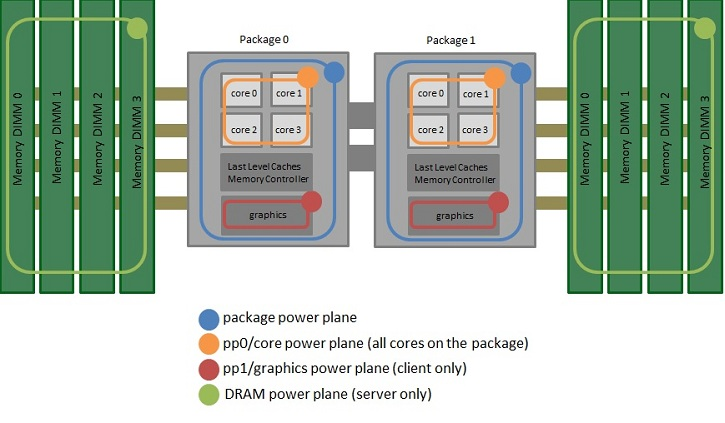
\includegraphics[width=\columnwidth]{images/power-planes-placeholder}
  \footnotesize{Source: "Intel® Power Governor" article\footnote{https://software.intel.com/en-us/articles/intel-power-governor}}
  \label{fig:power-planes}
\end{figure}
\end{savenotes}

With \ac{rapl}, developers can monitor energy consumption and set power limits. The access to this information is divided into different domains. Each domain is a physically meaningful domain for power management, as we can see in \figref{fig:power-planes}. The \ac{rapl} domains that are available in a platform vary across product segments. Typically, the desktop platforms have access to \{\texttt{PKG}, \texttt{PP0}, \texttt{PP1}\}, while the server platforms have access to \{\texttt{PKG}, \texttt{PP0}, \texttt{DRAM}\}. Each of these domains, provide fine-grained reports and control for power management. In \tabref{tbl:rapl-domains}, we show what each domain supports. For this work, we are interested in the \texttt{ENERGY\_STATUS} information as it provides the current measured energy consumption of a specific domain.

\begin{table}[htp]
	\centering
	\caption{List of controls supported by the RAPL domains}
	\rowcolors{1}{lightgray!30}{white}
	\begin{tabular}{ll}
	  \toprule
		\texttt{POWER\_UNIT}    & Provides the scaling factors for each unit\\
		\texttt{POWER\_LIMIT}   & Allows software to set power limits\\
		\texttt{ENERGY\_STATUS} & Reports measured actual energy usage\\
		\texttt{PERF\_STATUS}   & Reports the performance impact of power limiting\\
		\texttt{POWER\_INFO}    & Reports power range information for \ac{rapl} usage\\
	  \bottomrule
	\end{tabular}
	\label{tbl:rapl-domains}
\end{table}

The interaction with \acs{rapl} is done via \acp{msr}. Each control listed in \tabref{tbl:rapl-domains} for each domain is a separate \ac{msr}. \acp{msr} are special control registers present in the x86 instruction set that are typically used for debugging, monitoring performance, and toggling CPU features. Accessing \acp{msr} requires ring-0 access to the hardware, which is usually only allowed to the operating system kernel. This means that accessing the \ac{rapl} readings requires a kernel driver. In Linux, we do not have a specific driver to access the \ac{rapl} \acp{msr}. Instead, we have a generic \texttt{msr} driver (or kernel module) that exports \ac{msr} access to the userspace. The register readings are exposed as files inside the CPU device directories (e.g. \texttt{/dev/cpu/0/msr}). These files have read-only permission for superusers (root).

Manipulating these registers is not a very straightforward process. To do this, a developer need some knowledge of system programming and familiarity with the processor instruction set to know how to interpret the raw values exposed by the readings. Also, developers using \ac{rapl} need to handle possible register overflows. In a high power consumption scenario, for example, the \texttt{ENERGY\_STATUS} \ac{msr} of the \texttt{PKG} domain have a wraparound time of around 60 secs~\citep[p. 2465]{intel:2016}. So to abstract these low-level interfaces from Haskell developers, we present in the next sections two performance analysis tool that we extended to collect energy consumption information using \ac{rapl}.


\section{GHC Profiler}\label{sec:profiler}
A profiler is a tool for helping the development of efficient programs. Its main function is to provide the necessary information for developers to identify performance bottlenecks. So that once the hot spots in a program have been identified, the developer can work on the code to improve its performance and continuously check the effect of each modification. To achieve this goal, a profiler should keep track of important program resources. Moreover, the data gathered by the profiler must be related to the program source code in a way that is meaningful to the developer. This is usually accomplished by reporting the measurements by program structures (e.g. functions or methods) or source code structures (e.g. lines).

However, it is hard to establish this correspondence between measurements and source code for high-level languages. Usually, these languages provide abstractions and constructs that are unrelated to the way that the underlying execution engine works. Haskell is not different. Features such as polymorphism, high-order functions, and lazy evaluation make this task even harder. For example, in the presence of lazy evaluation, the evaluation of an expression can be interleaved with the evaluation of the inputs that this expression demands. This makes the resulting order of execution of expressions to bear no resemblance to the source code.

To address this problem, the \ac{ghc} profiler uses \emph{cost centres}~\citep{sansom:1995}. They are the logical components of the program to which the profiler associate the gathered data. A cost centre is simply a label to which we attribute execution costs. They are represented by annotations around expressions. So the costs incurred by the evaluation of the annotated expression are assigned to the enclosing cost centre. The cost centres can be automatically generated by the compiler or manually specified by the developer through the \texttt{\{-\# SCC \#-\}} directive. In \autoref{code:prof-mean}\footnote{This code example was extracted from \cite{sullivan:2008}}, we show an example of how it can be manually specified by the developer (line 10). In this example, all the costs incurred by the evaluation of \texttt{sum xs / fromIntegral (length xs)} will be attributed to the \texttt{mean} cost centre. It is important to point out that cost centres have a formally defined semantics~\citep{sansom:1995} that specifies how the cost attribution works.

\begin{listing}
  \caption{Haskell program to calculate the mean of a list of numbers}
  \begin{minted}{haskell}
import System.Environment
import Text.Printf

main :: IO ()
main = do
    [d] <- map read `fmap` getArgs
    printf "%f\n" (mean [1..d])

mean :: [Double] -> Double
mean xs = {-# SCC mean #-} sum xs / fromIntegral (length xs)
  \end{minted}
  \label{code:prof-mean}
\end{listing}

Currently, the \ac{ghc} profiler it is capable of measuring time and space usage. In \ac{ghc}, the profiler is part of the runtime system, which means that the profiling routines are contained within the final program executable. So to build a program for profiling, we need to pass to \ac{ghc} the \texttt{-prof} flag when compiling it. Then, to run this program in profiling mode, we need to specify it to the runtime system by passing the \texttt{+RTS -p} argument. It makes the runtime system collect time and memory usage data from the execution to produce a detailed report at the end. \figref{fig:profiler-sample} shows a profiling report for the program in \autoref{code:prof-mean}.

\begin{figure}[htp]
  \centering
  \caption{Example of profiling report for the \texttt{mean} program}
  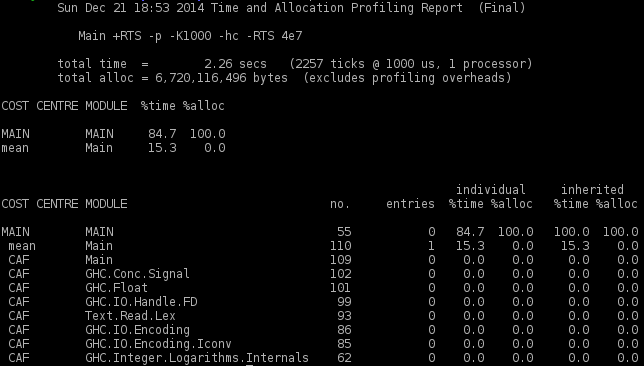
\includegraphics[width=\columnwidth]{images/profiler-placeholder}
  \footnotesize{Source: Generated by the GHC profiler}
  \label{fig:profiler-sample}
\end{figure}

As we can see in this example, we can split the report into three different sections. The first one is the header. It shows how the program was executed (which flags and arguments were passed to run it), and the total time and memory allocated during the whole execution of the program. The second part shows a break-down of the most costly cost centres. In this case, the top-level \texttt{MAIN} and the user-defined \texttt{mean}.

The third section shows a break-down by \emph{cost centre stack}~\citep{morgan:1998}. A cost centre stack is similar to a call graph. It defines a hierarchy of cost centres. In this case, we can see that \texttt{MAIN} is the root of the cost centre stack, followed by \texttt{mean} and some instances of \texttt{CAF} as children. A \ac{caf} is an expression that contains no free variables, i.e. it is a constant expression. So a \texttt{CAF} cost centre represents the one-off costs of evaluating such constants. Also, in this section of the report, we have multiple columns showing the profiling data. The time and memory usage percentage columns are shown into two different groups: \texttt{individual} and \texttt{inherited}. The former is the total of program resources spent by this cost centre while the latter is the total of program resources spent by this cost centre and its children. The other columns are \texttt{no.}, which is the id of the cost centre, and \texttt{entries}, which is the number of times that the expression enclosed by this cost centre was evaluated.

So to help on our journey of understanding the energy behavior of Haskell programs, we have extended the \ac{ghc} profiler to add a new metric: energy consumption. The idea is to collect energy consumption readings from \ac{rapl} and use the \ac{ghc} infrastructure to calculate the energy spent by each cost centre. Having this, we can display two new columns in the final report accounting the percentage of energy consumed by each cost centre. We based our solution on the approach used by the time profiler. To measure the execution time, the profiler keeps in each cost centre a tick counter. At any moment, the cost centre that is currently executing is held in a special register by the runtime system. Then, a regular clock interrupt\footnote{By default this interval is 20ms. However, the user can change it by passing a custom value to the runtime system via the \texttt{-V} argument.} runs a routine to increment this tick counter of the cost centre in execution. At the end of the program execution, the value held in the tick counter of each cost centre enables the profiler to determine and report the relative execution time cost of the different parts of the program.

Similarly, our extended version of the \ac{ghc} profiler keeps in each cost centre an accumulator. At each clock interrupt, the profiler adds to the accumulator of the cost centre that is currently in execution the energy consumed between the previous and current interrupt. This is accomplished by always saving the previous and current energy readings obtained from \ac{rapl}. If an overflow occurs on \ac{rapl} during the (extremely small) interval between two consecutive interrupts, we do not update the accumulator in this tick. At the end of the program execution, the profiler will be able to report the energy consumed by each cost centre based on its accumulator value. \figref{fig:energy-prof-report} shows the report of our extended GHC profiler the same program from \autoref{code:prof-mean}. As we can see in this report, we have now energy consumption information on each section of the report. In the header, we have the total energy consumed during the execution of the program. In the second and third sections, we have extra columns showing the percentage of energy consumed by each cost centres.

\begin{figure}[htp]
  \centering
  \caption{Example of profiling report with energy metrics for the \texttt{mean} program}
  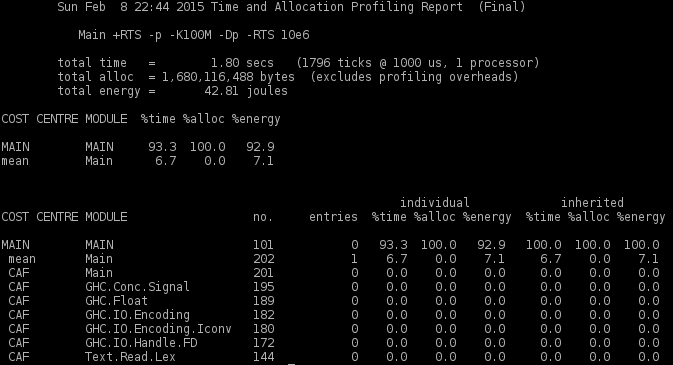
\includegraphics[width=\columnwidth]{images/energy-profiler-placeholder}
  \footnotesize{Source: Generated by the GHC profiler}
  \label{fig:energy-prof-report}
\end{figure}

Our modified version of \ac{ghc} is publicly available on GitHub\footnote{\url{http://github.com/green-haskell/ghc/tree/wip/green}}. It is based on \ac{ghc} 7.10 and includes the profiler with energy metrics. However, it is important to note that our implementation has one limitation. We can provide more accurate results only for programs that use a single capability. The main reason for this is the fact that \ac{rapl} does not provide the energy consumed by a single core. It provides only the energy consumption of the cores altogether, so if two cost centres are executing in parallel, we cannot tell how much energy each one consumed separately. However, we could easily adapt the current implementation to handle this case once the underlying \ac{api} provides the energy by core information. Also, it is easy enough to change the use of \ac{rapl} for another \ac{api} that provides energy consumption information if needed.

Despite this limitation, the profiler tool is particularly useful for providing fine-grained information about energy consumption. It enables developers to find the energy hot spots of Haskell programs. In the next section, we present another performance analysis tool called Criterion. Different from a profiler, it uses a coarse-grained approach for evaluating the performance of a program.


\section{Criterion}\label{sec:criterion}
Criterion~\citep{sullivan:2009} is a microbenchmarking library that is used to measure the performance of Haskell code. Its main objective is to estimate the cost of running a small, independent piece of code. At a first glance, it may seem that it does the same job of a profiler, but this is not the case. Criterion is not designed to finding hot spots in a program. Instead, it is useful for analyzing the cost of a given operation. A profiler is about taking a snapshot of a single execution of a program and reporting fine-grained information about its performance. Criterion, however, is about running a certain piece of code several times to analyze its performance. It reports to the developer a statistically-backed estimation of the cost of running the selected piece of code. As Criterion does not analyze the performance of each cost centre, only the benchmarked code as a whole, we say its analysis is coarse-grained.

Criterion provides a framework for both executing benchmarks as well as analysing their results. This framework is based on a simple \ac{api} that hides most of the complexity of performing benchmarks. In \autoref{code:fib-crit}\footnote{This example was extracted from \url{http://www.serpentine.com/criterion/tutorial.html}}, we show an example of how to define a Criterion benchmark. Here, we want to analyse the performance of the \texttt{fib} function. The benchmark is defined to execute \texttt{fib} passing 9 as argument. We provide the Criterion \ac{api} in details on \appref{ap:criterion}. Here in this example, we are using three important function of its \ac{api}:
\begin{itemize}
  \item \texttt{defaultMain}: takes care of executing a set of benchmarks
  \item \texttt{bench}: creates a benchmark based on an action provided by the developer
  \item \texttt{whnf}: makes sure the benchmarked action is evaluated to weak head normal form to avoid it to be evaluated only once due to Haskell's laziness
\end{itemize}

\begin{listing}
  \caption{Definition of a Criterion benchmark for the \texttt{fib} function}
  \begin{minted}{haskell}
import Criterion.Main

fib :: Int -> Int
fib m | m < 0     = error "negative!"
      | otherwise = go m
  where
    go 0 = 0
    go 1 = 1
    go n = go (n-1) + go (n-2)

main :: IO ()
main = defaultMain [
    bench "fib/9" (whnf fib 9)
  ]
  \end{minted}
  \label{code:fib-crit}
\end{listing}

In \figref{fig:fib-output}, we show the output for the benchmark described by \autoref{code:fib-crit}. The first line shows \texttt{time}, which is the estimation of the time needed for executing \texttt{fib 9} once. It is obtained using an \ac{ols} regression model. Inside the parenthesis, after the time estimation, we can see the lower and upper bounds of the confidence interval that is calculated using \emph{bootstrapping}~\citep{davison:1997}. It means that when randomly resampling the data, 95\% of estimates fell between the lower and upper bounds of the interval. So the quality of the estimation is better when the bounds are closer to its value. The second line shows the coefficient of determination, or R\textsuperscript{2}, which is a statistical measure of how well the linear regression model approximates the observed measurements. An R\textsuperscript{2} between 0.99 and 1 indicates an excelent approximation. The \texttt{mean} and \texttt{std dev} lines are the mean execution time and the standard deviation, respectively. Finally, the last line indicates the degree to which the standard deviation is inflated by outlying measurements.

\begin{figure}[htp]
  \centering
  \caption{Output of the \texttt{fib} benchmark}
  \begin{minted}{text}
benchmarking fib/9
time                 314.4 ns   (312.2 ns .. 318.5 ns)
                     0.999 R²   (0.997 R² .. 1.000 R²)
mean                 315.3 ns   (314.0 ns .. 319.4 ns)
std dev              7.081 ns   (1.625 ns .. 14.63 ns)
variance introduced by outliers: 26% (moderately inflated)
  \end{minted}
  \footnotesize{Source: Generated by Criterion}
  \label{fig:fib-output}
\end{figure}

This kind of information that Criterion provides is quite useful for making sure that the measurements are not being tainted by external factors such as other loads on the operating system. Alongside with the textual report, Criterion can also generate some charts like the one shown in \figref{fig:crit-chart}. In this chart, the $x$-axis indicates the number of loop iterations, while the $y$-axis shows the execution time for a given number of iterations. The blue circles are the raw measurements while the orange line is the linear regression generated from this data. The closer the dots are from the line, the better is the regression model.

\begin{figure}[htp]
  \centering
  \caption{Measurement chart generated for the \texttt{fib} benchmark}
  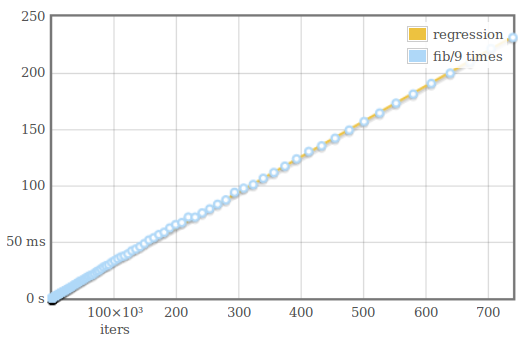
\includegraphics[width=.6\columnwidth]{images/criterion-chart} \\
  \footnotesize{Source: Generated by Criterion}
  \label{fig:crit-chart}
\end{figure}

As we can see from this example, each sample that Criterion uses for the regression model corresponds to the measurements collected during a distinct number of consecutive executions of the benchmarked code. This specific number of loop iterations is the independent variable of the regression model, which the author calls \texttt{iters}. The number of different \texttt{iters} that Criterion performs for a given benchmark depends on how much time the benchmarked code takes to run. Criterion tries to run it as much as possible so that: (1) it collects enough measurements for properly resampling the data; and (2) it generates enough measurements that have long spans of execution to outweigh the cost of measurement. For short-lived benchmarks such as \autoref{code:fib-crit}, in the order of nanoseconds, we can see that Criterion collects several samples with a high number of consecutive iterations. For longer benchmarks, in the order of tens of seconds, it is garanteed that Criterion will collect at least five samples, from one to five iterations each, respectively\footnote{This information is not available on the library documentation. We got it by inspecting the source code.}.

\begin{figure}[htp]
  \centering
  \caption{Output with CPU cycles of the \texttt{fib} benchmark}
  \begin{minted}{text}
benchmarking fib/9
time                 317.2 ns   (314.2 ns .. 319.4 ns)
                     0.999 R²   (0.999 R² .. 1.000 R²)
mean                 314.4 ns   (313.3 ns .. 315.8 ns)
std dev              4.117 ns   (2.682 ns .. 5.398 ns)
cycles:              0.999 R²   (0.999 R² .. 1.000 R²)
  iters              1079.434   (1069.292 .. 1087.144)
  y                  924904.370 (562772.048 .. 1358678.998)
variance introduced by outliers: 13% (moderately inflated)
  \end{minted}
  \footnotesize{Source: Generated by Criterion}
  \label{fig:fib-cycle-output}
\end{figure}

Besides elapsed time, Criterion can also perform linear regression on other metrics such as CPU time, CPU cycles, bytes allocated and number of garbage collections. It can be done by passing the other metric as a command line argument when running the benchmark. For example, passing \texttt{-{}-regress cycles:iters} will regress the number of CPU cycles against the number of loop iterations. \figref{fig:fib-cycle-output} shows the output for such example for \autoref{code:fib-crit}. As we can see, we have three extra lines on the report. The first one corresponds to the R\textsuperscript{2} for the new regression we specified. The second line we have the estimation of how much cycles each iteration costs, which is the slope of the regression curve. The last line is where the curve intercepts the $y$-axis. This feature allows for developers to have a good overview from different perspectives about the performance of the benchmarked code.

In order to employ Criterion in our work, we have extended it to add a new metric: energy consumption. The fact that Criterion's infrastructure already have support for estimating the cost of other metrics than elapsed time helped us to modify it in a "cleaner" way. However, the way the energy data is collected is different from the other metrics due to the fact that \ac{rapl} registers are susceptible to overflows. In \autoref{code:crit-measure}, we show how Criterion currently collects the measurements data. As we can see, it saves the counters before and after it executes the benchmarked code \texttt{iters} times. If we used the same approach for energy consumption, in the presence of an overflow, the data collected would be inconsistent.

\begin{listing}
  \caption{Internal function that execute the benchmarks in Criterion}
  \begin{minted}{haskell}
measure :: Benchmarkable -> Int64 -> IO (Measured, Double)
measure (Benchmarkable run) iters = do
  startStats <- getGCStats
  startTime <- getTime
  startCpuTime <- getCPUTime
  startCycles <- getCycles
  run iters
  endTime <- getTime
  endCpuTime <- getCPUTime
  endCycles <- getCycles
  endStats <- getGCStats
  let !m = applyGCStats endStats startStats $ measured {
             measTime    = max 0 (endTime - startTime)
           , measCpuTime = max 0 (endCpuTime - startCpuTime)
           , measCycles  = max 0 (fromIntegral (endCycles - startCycles))
           , measIters   = iters }
  return $ (m, endTime)
  \end{minted}
  \label{code:crit-measure}
\end{listing}

To overcome this problem, we collect the energy consumption slightly different from the other metrics. We have to constantly read the \ac{rapl} counters during the benchmark execution in order to detect overflows. One way we could accomplish this task is by spawning a background thread to collect the energy data. However, this is approach is not very lightweight. It would increase the measurement overhead and possibly influence the result of more sensitive benchmarks. So instead, we have used native Linux signals. So it works as following: before Criterion runs the benchmarked code, we register a Linux signal to be fired every 10ms. When registering this signal, we attach a signal handler that we implemented. Inside this handler, we read the \ac{rapl} counters, check if an overflow happened, and if not, we save the energy consumed between the last two readings into an internal accumulator. At the end, when the benchmark finishes executing, we can deregister the signal and get the value hold by the accumulator, which is the energy measurements.

To implement this solution, similarly to how the time and cycles data is collected, we use native C code. The communication with the Criterion code, which is implemented in Haskell, is done straightforwardly via foreign function interface (FFI) calls. The interface with Linux to use signals is done using the \texttt{sigaction} and \texttt{setitimer} syscalls. The source code of our modifed version of Criterion is publicly available on GitHub\footnote{\url{http://github.com/green-haskell/criterion}}. In \figref{fig:fib-energy-output}, we show an example of output with the energy metrics for a benchmark we used the study presented in the next chapter. In this case, a single execution of the program is expected to consume 180.9 joules of energy.

\begin{figure}[htp]
  \centering
  \caption{Output example of Criterion with energy metrics}
	\begin{minted}{text}
benchmarking dining-philosophers (forkOS | MVar)
time                 2.183 s    (1.915 s .. 2.510 s)
                     0.997 R²   (0.991 R² .. 1.000 R²)
mean                 2.179 s    (2.113 s .. 2.212 s)
std dev              57.17 ms   (0.0 s .. 57.19 ms)
energy:              0.999 R²   (0.997 R² .. 1.000 R²)
  iters              180.947    (164.629 .. 200.826)
  y                  0.937      (-71.359 .. 37.230)
variance introduced by outliers: 19% (moderately inflated)
  \end{minted}
  \footnotesize{Source: Generated by Criterion}
  \label{fig:fib-energy-output}
\end{figure}

As we can see, Criterion is a powerful tool. It provides a robust methodology for performing benchmarks of Haskell code. In the next chapter, we present an empirical study where Criterion was heavly employed to measure the performance and energy consumption of various concurrent programming constructs.

\chapter{The Energy Efficiency of Concurrent Haskell}
In this chapter, we present an empirical study evaluating the performance and energy consumption characteristics of three thread management constructs and three data-sharing primitives of Concurrent Haskell. We start by providing a brief overview (\secref{sec:overview}) of the study and state the research questions. \secref{sec:setup} describes the benchmark we developed, the environment and the methodology we used. Sections \ref{sec:results} and \ref{sec:discussion} provides our results. Finally, \secref{sec:threats} list the threats to validity.

\section{Overview}\label{sec:overview}
Recently, the software engineering community have been showing a keen interest in researching about the development of energy-efficient software. As multicore architectures are the norm nowadays, this interest also extends for energy-efficiency from the perspective of concurrent software running on multicore architectures~\citep{trefethen:2013,ribic:2014, pinto:2014}. However, there is no much traction from the functional programming side yet. This is unfortunate as functional programming languages are seen as a good alternative for making concurrent programming less error-prone. Particularly, Haskell provides a solid foundation for building concurrent software, and we know very little about its energy behavior.

We believe that the first step to optimizing energy consumption of concurrent programs is to gain a comprehensive understanding of their energy behaviors. This chapter presents an empirical study to understand the energy behaviors of Haskell concurrent programs on multicore architectures. In particular, our study focuses on how programmer's decisions may impact energy consumption and performance. The following questions motivate our research:

\begin{enumerate}[label=\RQ{\arabic*}.]
  \item Do alternative \textit{thread management constructs} have different impacts on energy consumption?
  \item Do alternative \textit{data-sharing primitives} have different impacts on energy consumption?
  \item What is the relationship between the \textit{number of capabilities} and energy consumption?
\end{enumerate}

To answer \RQ{1}, we select three thread management constructs: \forkIO, \forkOn and \forkOS. As we saw in \secref{sec:haskell-conc}, these are the three functions we have in Haskell to spawn a new thread of execution. To answer \RQ{2}, we select three data-sharing primitives: \MVar, \TMVar and \TVar. Given these constructs, our investigation aims to understand how the energy consumption can be impacted by simply changing the concurrency primitive used in a Haskell program. Finally, to answer \RQ{3}, we explore various capabilities settings to see how it can impact energy consumption and performance on a multicore environment.


\section{Study Setup}\label{sec:setup}
In this section we describe the benchmarks that we analyzed, the infrastructure and the methodology that we used to perform the experiments.

\subsection{Benchmarks}
We selected a variety of concurrent Haskell programs to use as benchmarks in our study, listed as follows. Benchmarks \ref{bench:chameneos}-\ref{bench:spectral} are from \ac{clbg}\footnote{http://benchmarksgame.alioth.debian.org/}. \acs{clbg} is a benchmark suite aiming to compare the performance of the runtime of various programming languages. Benchmark \ref{bench:dining} is from  Rosetta Code \footnote{http://rosettacode.org/}, a code repository of solutions to common programming tasks. Benchmarks \ref{bench:tsearch}-\ref{bench:warp} were developed by us.

\begin{enumerate}
  \item \label{bench:chameneos}\chameneos: In this benchmark chameneos creatures go to a meeting place and exchange colors with a meeting partner. It encodes symmetrical cooperation between threads.

  \item \fasta:  This benchmark generates random DNA sequences and writes it in FASTA format\footnote{https://en.wikipedia.org/wiki/FASTA\_format}. The size of the generated DNA sequences is in the order of hundreds of megabytes. In this benchmark,  each worker synchronizes with the previous one to output the sub-sequences of DNA in the correct order.

  \item \knucleotide: This benchmark takes a DNA sequence and counts the occurrences and the frequency of nucleotide patterns. This benchmark employs string manipulation and hashtable updates intensively. There is no synchronization in the program besides the main thread waiting for the result of each worker.

  \item \mandelbrot: A mandelbrot is a mathematical set of points whose boundary is a distinctive and easily recognizable two-dimensional fractal shape. Mandelbrot set images are created by sampling complex numbers and determining for each one whether the result tends toward infinity when a particular mathematical operation is iterated on it. The only synchronization point in this benchmark is the main thread waiting for the result of each worker.

  \item \regex: This benchmark implements a string-based algorithm that performs multiple regular expression operations, match and replace, over a DNA sequence. The only synchronization point is the main thread waiting for the result of each worker.

  \item \label{bench:spectral}\spectral: The spectral norm is the maximum singular value of a matrix. It synchronizes the workers using a cyclic barrier.

  \item \label{bench:dining}\dining: An implementation of the classical concurrent programming problem posed by~\cite{dijkstra:1971}. The philosophers perform no work besides manipulating the forks and printing a message when eating.

  \item \label{bench:tsearch}\tsearch: A parallel text search engine. This benchmark searches for occurrences of a sentence in all text files in a directory and its sub-directories. It is based on a previous empirical study comparing STM and locks~\citep{pankratius:2011}.

  \item \label{bench:warp}\warp: Runs a set of queries against a Warp server retrieving the resulting webpages. Warp is the default web server used by the \ac{wai}, part of the Yesod Web Framework. This benchmark was inspired by the Tomcat benchmark from DaCapo~\citep{blackburn:2006}.
\end{enumerate}

We selected the benchmarks based on their diversity. For instance, \chameneos and \dining are synchronization-intensive programs. \mandelbrot and \spectral are CPU-intensive and scale well on a multicore machine. \knucleotide and \regex are CPU- and memory-intensive, while \warp is IO-intensive. \tsearch combines IO and CPU operations, though much of the work it performs is CPU-intensive. \fasta is peculiar in that is CPU-, memory-, synchronization- and IO-intensive.

Also, some benchmarks have a fixed number of workers (\chameneos, \knucleotide, \regex, and \dining) and others spawn as many workers as the number of capabilities (\fasta, \mandelbrot, \spectral, \tsearch and \warp). For the \dining benchmark, it is possible to establish prior to execution the number of workers.

\subsection{Experimental Environment}
For our study, all experiments were conducted on a machine with 2x10-core Intel Xeon E5-2660 v2 processors (Ivy Bridge microarchitecture), 2.20 GHz, with 256GB of DDR3 1600MHz memory. It has three cache levels (L1, L2, L3): L1 with 32KB per core, L2 with 256KB per core, and L3 with 25MB per socket (Smart cache). This machine runs the Ubuntu Server 14.04.3 LTS (kernel 3.19.0-25) operating system, \acs{ghc} 7.10.2, and our modified Criterion based on version 1.1.0 of the official release.

All experiments were performed with no other load on the OS. We conform to the default settings of the operating system. For each benchmark, we used the same compilation and runtime flags employed in the original benchmark suites. This is important to preserve the same performance characteristics as intended by the implementers. Both the energy consumption and the performance is measured by Criterion.

\subsection{Methodology}
Most of the benchmarks we used were implemented in its respective suite using a single thread management construct and a single data-sharing primitive. For the ones from \acs{clbg}, for example, they were implemented using \forkIO and \MVar. In order to analyze the impact of both thread management constructs and data-sharing primitives, we manually refactored each benchmark to create new \emph{variants} using different constructs. Changing the thread management construct is a straightforward process. The functions have almost the same signature. The only exception is \forkOn that requires an extra argument representing in which capability the thread will run. For this study, we distributed the threads evenly among the capabilities when using \forkOn. However, changing the data-sharing primitive is not always simple as a \TVar have a quite different semantics when compared to an \MVar. To properly do this refactoring, we used the techniques proposed by~\cite{soares-neto:2014} to refactor the benchmarks to use STM.

As a result of this process, each benchmark has up to 9 distinct variants covering a number of different combinations of both thread management constructs and data-sharing primitives. However, it is important to note that there are some cases like \dining where not all possible combinations were created. In this particular implementation, the shared variable is also used as a condition-based synchronization mechanism. In such cases, we did not create \TVar variants as \TMVar mimics exactly this behavior, while using Haskell's STM. In other benchmarks like \tsearch and \warp, we changed only the thread management construct as they are complex applications and it would not be straightforward to change the synchronization primitives without introducing potential bugs.

In the end, each variant we created is represented by a standalone executable. This executable is a Criterion microbenchmark that performs the experiment by calling the original program entry point multiple times. We run this executable nine times, each one changing the number \texttt{N} of capabilities used by the runtime system. We used the following values for \texttt{N}: $\{1, 2, 4, 8, 16, 20, 32, 40, 64\}$. Where 20 and 40 are the number of physical and virtual cores, respectively.

In \appref{ap:benchmark}, we provide an example of one of the benchmarks we used. We show the description of the problem that this benchmark solves and the implementation of each variant we generated to use in this study. It can also be accessed on GitHub at \url{http://github.com/green-haskell/concurrency-benchmark}. In this repository, we made publicly available the implementation of all benchmarks variants as well as the scripts and instructions necessary to replicate this experiment.


\section{Study Results}\label{sec:results}
In this section, we report the results of our experiments with concurrent Haskell programs. The results are presented in Figures \ref{fig:conc_bench1}, \ref{fig:conc_bench2} and \ref{fig:conc_bench3}. Here, the odd rows are energy consumption results, while the even rows are the corresponding running time results. We omitted the experiments using 64 capabilities in order to make the charts more readable. The charts including this configuration as well as all the data and source code used in this study are available at \href{http://green-haskell.github.io/}{green-haskell.github.io}.
\newline

\begin{figure*}[tp]
\caption{Energy and Time charts for \chameneos, \dining, \fasta and \knucleotide}
\centering
$
\begin{array}{ccc}
 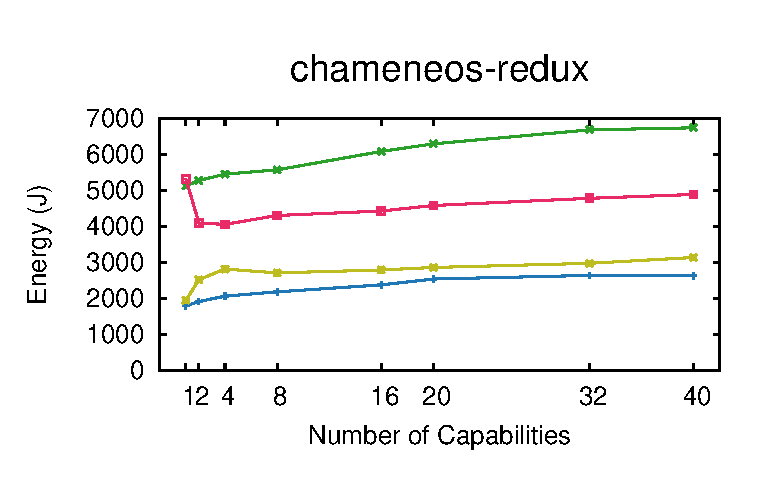
\includegraphics[width=.48\textwidth]{images/conc_bench/chameneos-redux-energy} &
 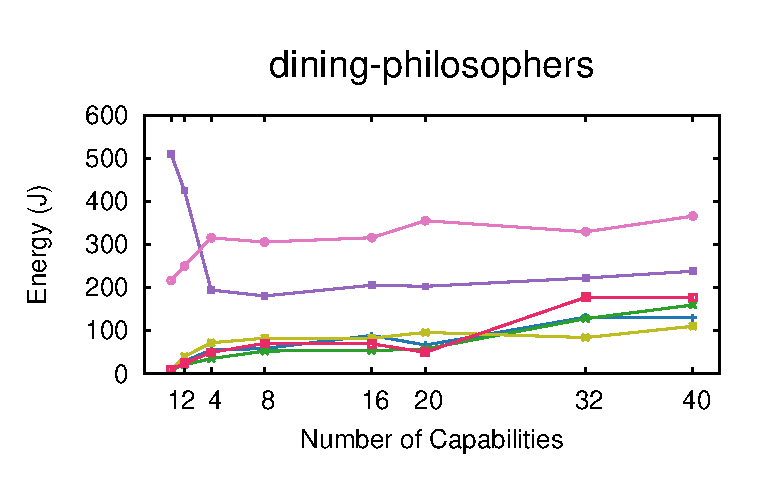
\includegraphics[width=.48\textwidth]{images/conc_bench/dining-philosophers-energy} \\
 \\

 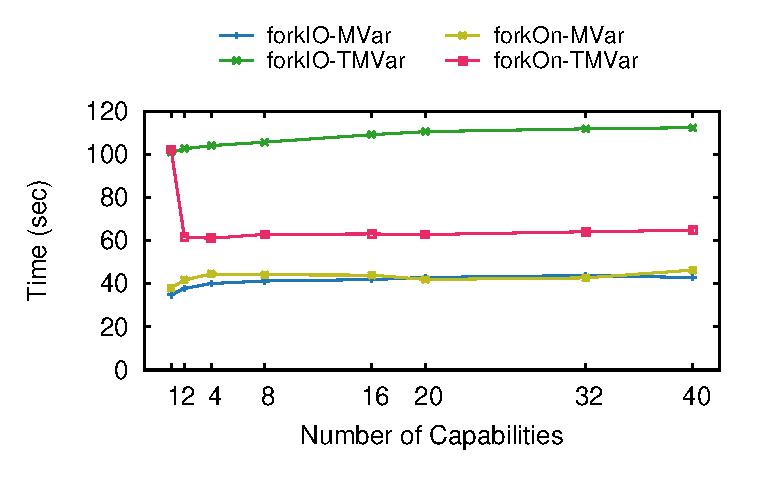
\includegraphics[width=.48\textwidth]{images/conc_bench/chameneos-redux-time} &
 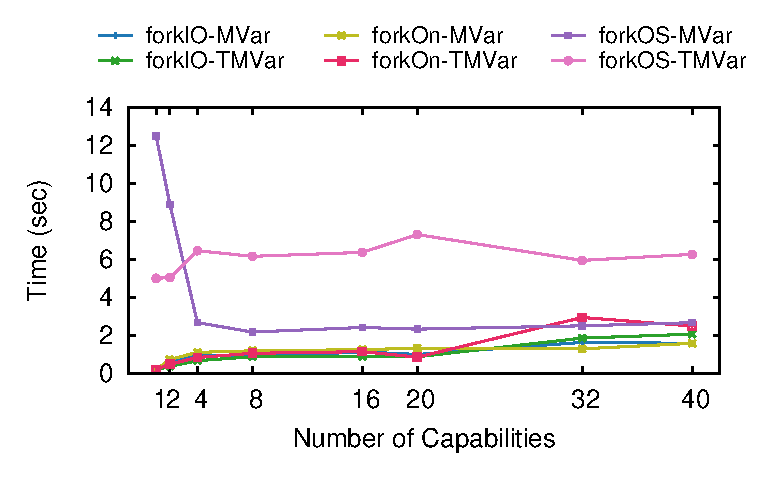
\includegraphics[width=.48\textwidth]{images/conc_bench/dining-philosophers-time} \\

 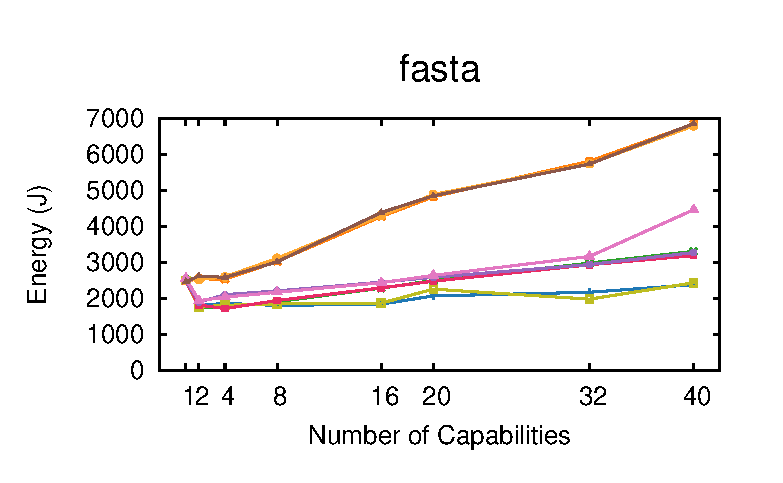
\includegraphics[width=.48\textwidth]{images/conc_bench/fasta-energy} &
 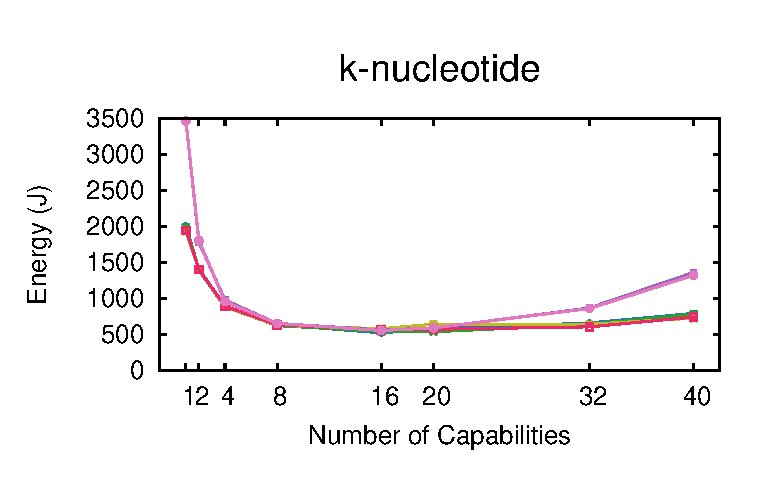
\includegraphics[width=.48\textwidth]{images/conc_bench/k-nucleotide-energy}  \\

 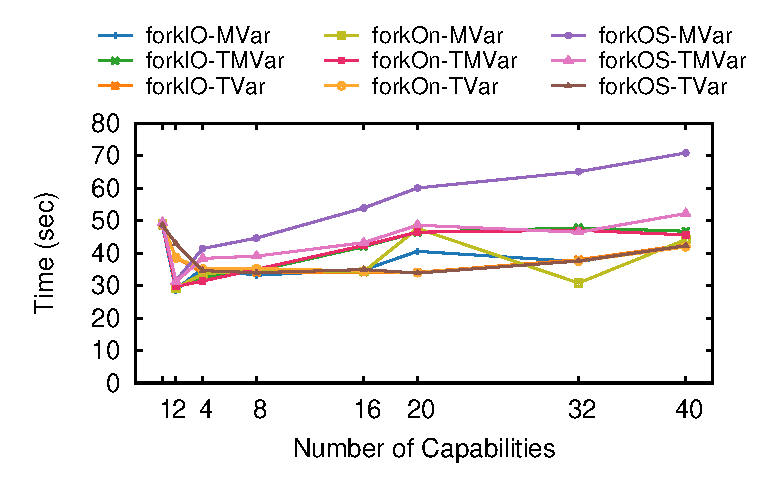
\includegraphics[width=.48\textwidth]{images/conc_bench/fasta-time} &
 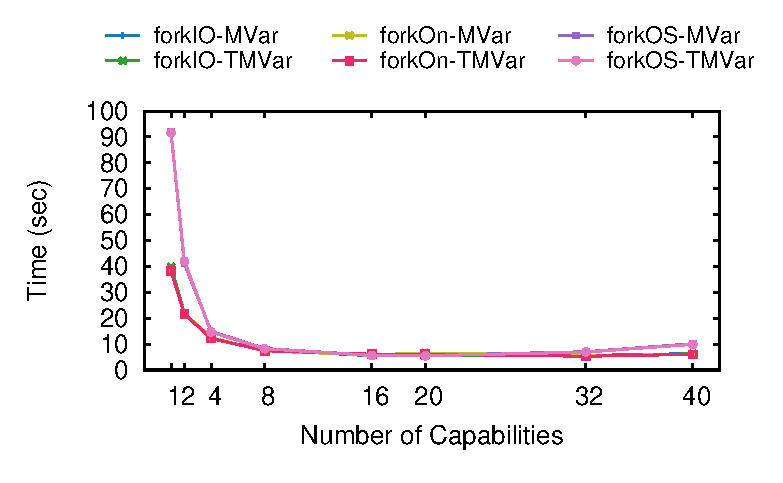
\includegraphics[width=.48\textwidth]{images/conc_bench/k-nucleotide-time}  \\
\end{array}
$
\footnotesize{Source: Made by the author.}
\label{fig:conc_bench1}
\end{figure*}

\begin{figure*}[tp]
\caption{Energy and Time charts for \mandelbrot, \regex, \spectral and \tsearch}
\centering
$
\begin{array}{ccc}
 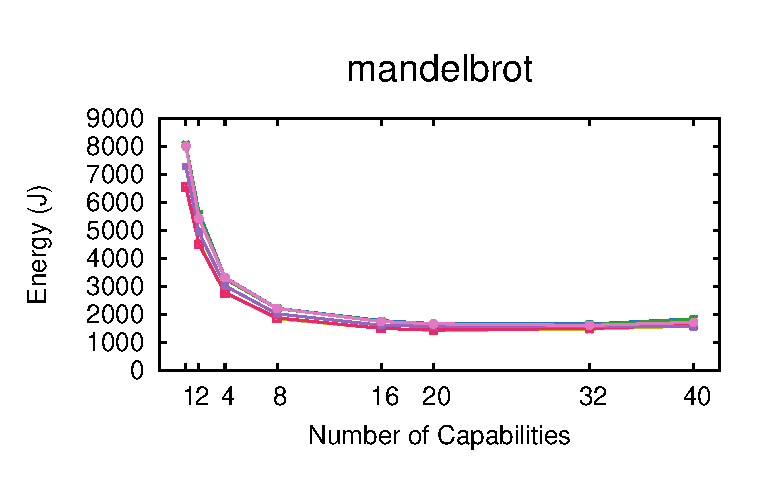
\includegraphics[width=.48\textwidth]{images/conc_bench/mandelbrot-energy} &
 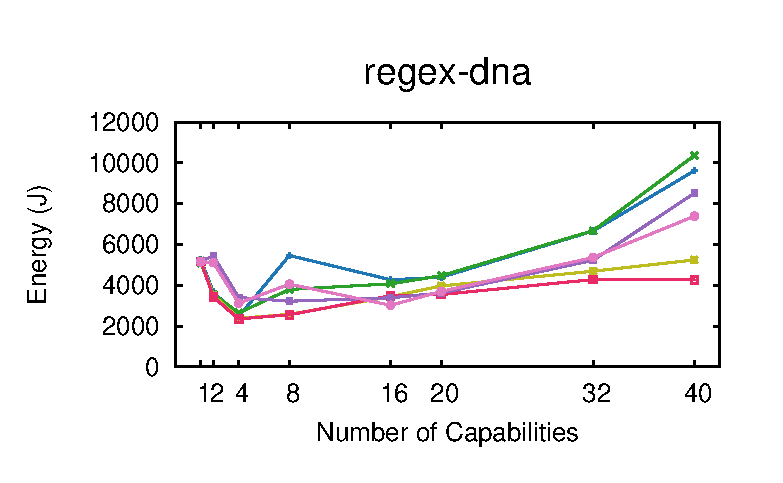
\includegraphics[width=.48\textwidth]{images/conc_bench/regex-dna-energy} \\

 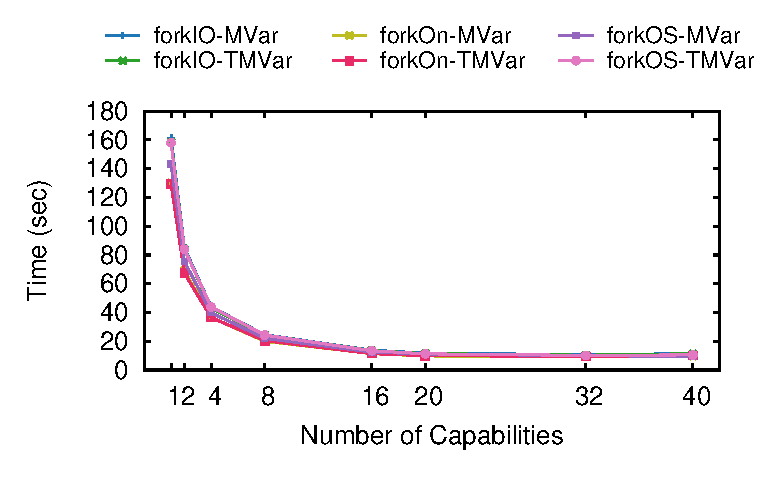
\includegraphics[width=.48\textwidth]{images/conc_bench/mandelbrot-time} &
 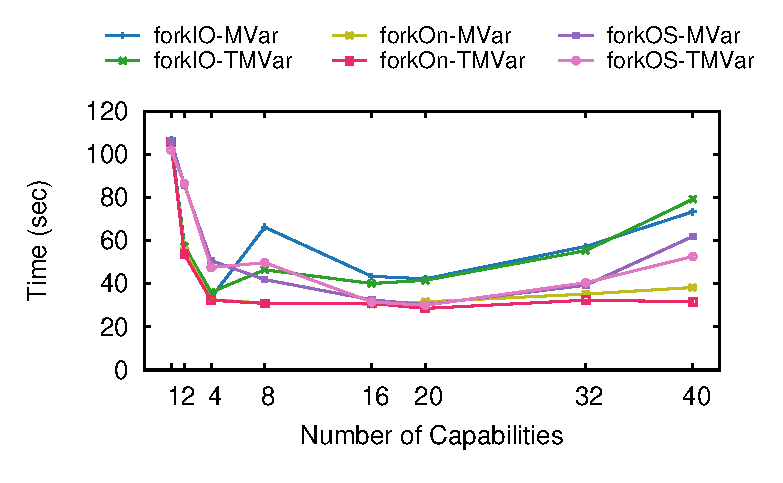
\includegraphics[width=.48\textwidth]{images/conc_bench/regex-dna-time} \\
 \\

 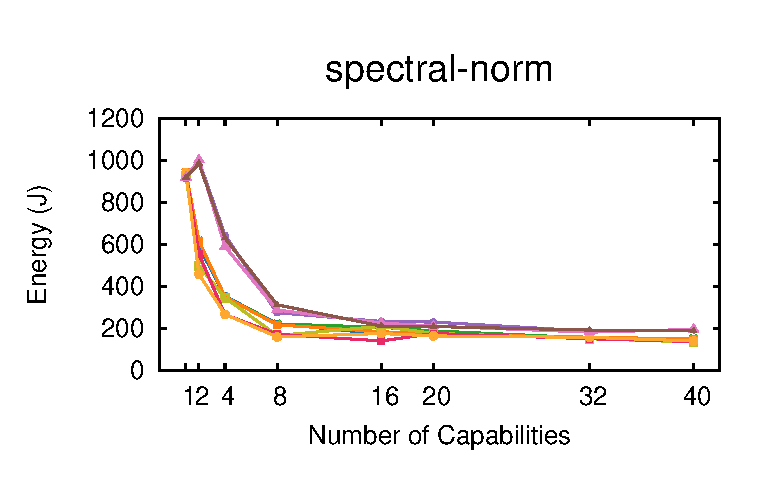
\includegraphics[width=.48\textwidth]{images/conc_bench/spectral-norm-energy} &
 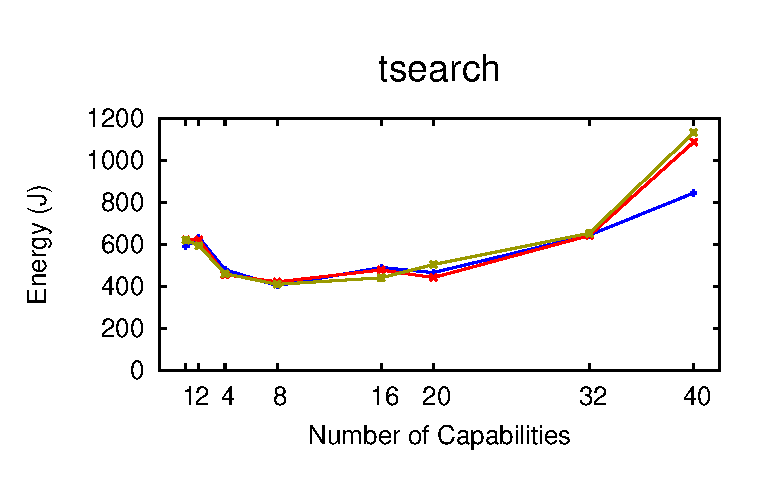
\includegraphics[width=.48\textwidth]{images/conc_bench/tsearch-energy} \\

 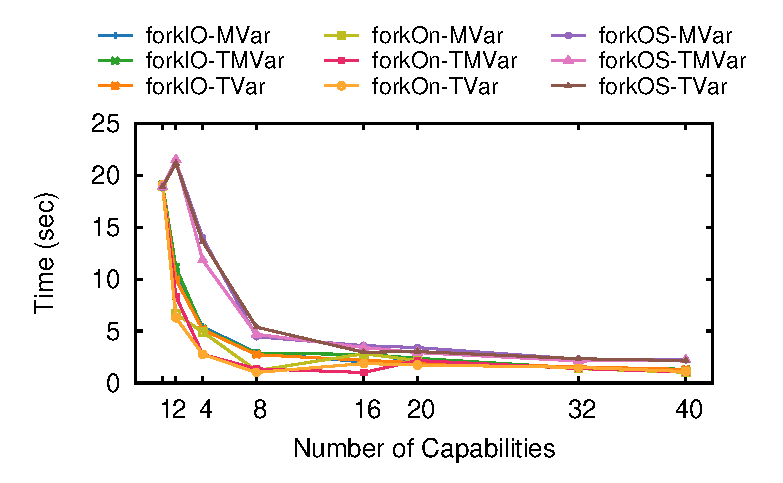
\includegraphics[width=.48\textwidth]{images/conc_bench/spectral-norm-time} &
 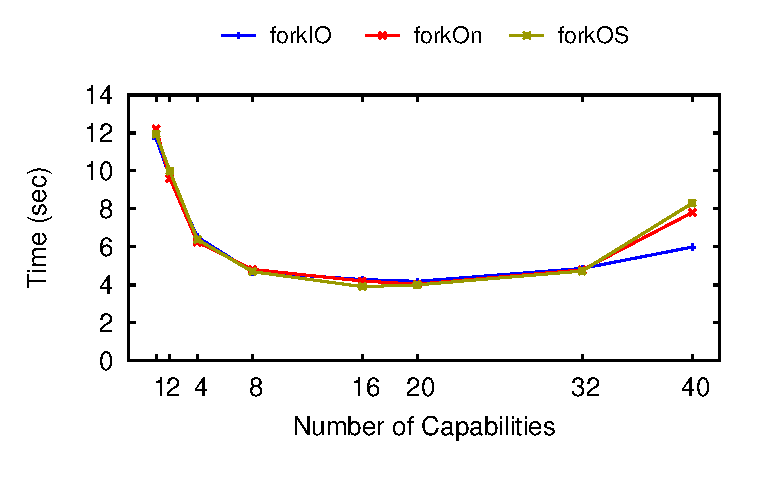
\includegraphics[width=.48\textwidth]{images/conc_bench/tsearch-time} \\
\end{array}
$
\footnotesize{Source: Made by the author.}
\label{fig:conc_bench2}
\end{figure*}

\begin{figure*}[tp]
\caption{Energy and Time charts for \warp}
\centering
$
\begin{array}{c}
 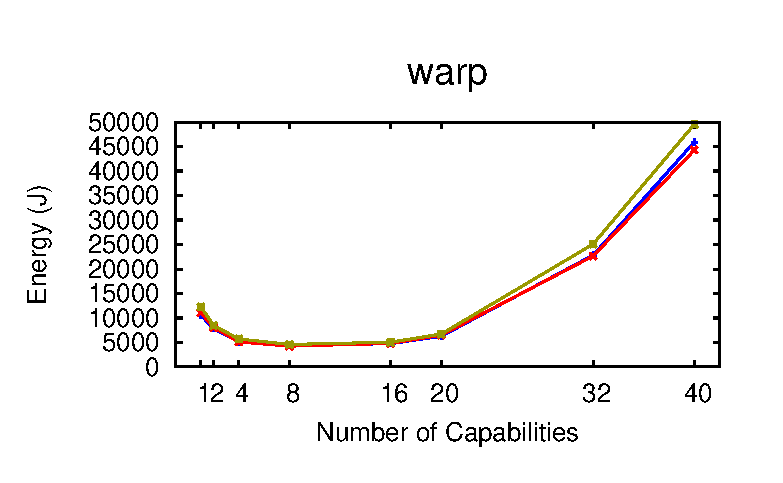
\includegraphics[width=.48\textwidth]{images/conc_bench/warp-energy} \\
 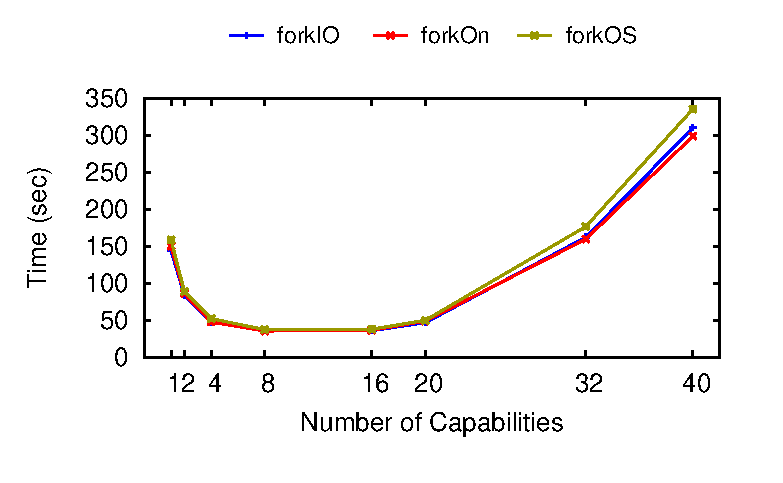
\includegraphics[width=.48\textwidth]{images/conc_bench/warp-time} \\
\end{array}
$
\\
\footnotesize{Source: Made by the author.}
\label{fig:conc_bench3}
\end{figure*}

\state{Small changes can produce big savings.} One of the main findings of this study is that simple refactorings such as switching between thread management constructs can have considerable impact on energy usage. For example, in \spectral, using \forkOn instead of \forkOS with \TVar can save between 25 and 57\% energy, for a number of capabilities ranging between 2 and 40. Although the savings vary depending on the number of capabilities, for \spectral \forkOn exhibits lower energy usage independently of this number. For \mandelbrot, variants using \forkOS and \forkOn with \MVar exhibited consistently lower energy consumption than ones using \forkIO, independently of the number of capabilities. For the \forkOS variants, the savings ranged from 5.7 to 15.4\% whereas for \forkOn variants the savings ranged from 11.2 to 19.6\%.

This finding also applies to data sharing primitives. In \chameneos, switching from \TMVar to \MVar with \forkOn can yield energy savings of up to 61.2\%. Moreover, it is advantageous to use \MVar independently of the number of capabilities. In a similar vein, in \fasta, going from \TVar to \MVar with \forkIO can produce savings of up to 65.2\%. We further discuss the implications of this finding in \secref{sec:discussion}.
\newline

\state{Faster is not always greener.} Overall, the shapes of the curves in Figures \ref{fig:conc_bench1}, \ref{fig:conc_bench2} and \ref{fig:conc_bench3} are similar. Although, for 6 of our 9 benchmarks, in at least two variants of each one, there are moments where faster running time leads to a higher energy consumption. For instance, in the \forkOn-\TMVar variant of \regex, the benchmark is 12\% faster when varying the number of capabilities from 4 to 20 capabilities. But at the same time, its energy consumption increases by 51\% . Also, changing the number of capabilities from 8 to 16 in the \forkIO variant of \tsearch makes it 8\% faster and 22\% less energy-efficient.

In one particular benchmark, \fasta, we had strongly divergent results in terms of performance and energy consumption for some of the variants. For this benchmark, the variants  employing \TVar outperformed the ones using \TMVar and \MVar. For example, when using a number of capabilities equal to the number of physical cores of the underlying machine (20), the \forkOS-\TVar variant was 43.7\% faster than the \forkOS-\MVar one. At the same time, the \TVar variants exhibited the worst energy consumption. In the aforementioned configuration, the \forkOS-\TVar variant consumed 87.4\% more energy.
\newline

\state{There is no overall winner.} Overall, no thread management construct or data sharing primitive, or combination of both is the best. For example, the \forkIO-\TMVar variant is one of most energy-efficient for \dining. The \forkOS-\TMVar variant consumes more than 6 times more energy. However, for the \chameneos benchmark, the \forkIO-\TMVar variant consumes 2.4 times more energy than the best variant, \forkIO-\MVar. This example is particularly interesting because these two benchmarks have similar characteristics. Both \dining and \chameneos are synchronization-intensive benchmarks and both have a fixed number of worker threads. Even in a scenario like this, using the same constructs can lead to discrepant results.
\newline

\state{Choosing more capabilities than available CPUs is harmful.} The performance of most benchmarks is severely impaired by using more capabilities than the number of available CPUs. In \chameneos, for example, moving from 40 to 64 capabilities can cause a 13x slowdown. This suggests that the Haskell runtime system was not designed to handle cases where capabilities outnumber CPU cores. In fact, this assumption makes sense as the official GHC documentation recommends the number of capabilities to match the number of CPU cores. However, the documentation leaves as an open question if virtual cores should be counted. In our experiments, the performance almost never improves after 20 capabilities. So developers should be careful when using more capabilities than available physical CPU cores as it can degrade performance.


\section{Discussion}\label{sec:discussion}
Generally, especially in the sequential benchmarks, high performance is a proxy for low energy consumption. A study we published \citep{lima:2016} highlighted this for a number of different data structure implementations and operations. Concurrency makes the relationship between performance and energy less obvious, however. Also, there are clear benefits in employing  different thread management constructs and data-sharing primitives. This section examines this in more detail.

Switching between thread management construct is very simple in Haskell. Functions \forkOn, \forkIO, and \forkOS take a computation of type \IO as parameter and produce results of the same type. Thus, the only difficulty is in determining on which capability a thread created via \forkOn will run. This is good news for developers and maintainers. Considering the 7 benchmarks where we implemented variants using different data sharing primitives, in 5 of them the thread management construct had a stronger impact on energy usage than the data sharing primitives. Furthermore, in these 5 benchmarks and also in \warp it is clearly beneficial to switch between thread management constructs.

Alternating between data sharing primitives is not as easy, but still not hard, depending on the characteristics of the program to be refactored. Going from \MVar to \TMVar and back is straightforward because they have very similar semantics. The only complication is that, since functions operating on \TMVar produce results of type \STM, calls to these functions must be enclosed in calls to \atomically to produce a result of type \IO. Going from \MVar to \TVar and back is harder, though. If a program using \MVar does not require condition-based synchronization, it is possible to automate this transformation in a non-application-dependent manner~\citep{soares-neto:2014}. If condition-based synchronization is necessary, such as is the case with the \dining benchmark, the semantic differences between \TVar and \MVar make it necessary for the maintainer to understand details of how the application was constructed.

In spite of the absence of an overall winning thread management construct or data-sharing primitive, we can identify a few cases where {\em a specific approach excels under specific conditions}. For instance, we can see that in both \mandelbrot and \spectral, \forkOn has a slightly better performance than \forkIO and \forkOS. In \mandelbrot, the \forkOn variants are around 20\% more energy-efficient than the \forkIO variants. In \spectral, \forkOn can be up to 2x greener than \forkOS. These two benchmarks are both CPU-intensive. They also create as many threads as the number of capabilities. In a scenario such as this, a computation-heavy algorithm with few synchronization points, keeping each thread executing in a dedicated CPU core is beneficial for the performance. This is precisely what \forkOn does.

Although there is no overall winner, there is a more or less clear loser, when thread management construct have a strong impact on energy: \forkOS. In only one of the benchmarks the \forkOS variants did not have the worst energy consumption and worst performance: \regex. According to the Haskell documentation\footnote{https://hackage.haskell.org/package/base-4.8.1.0/docs/Control-Concurrent.html\#v:forkOS}: \emph{"Using forkOS instead of forkIO makes no difference at all to the scheduling behavior of the Haskell runtime system".} If that is the case, the extra time and energy consumption stem from the need to switch OS threads to execute work passed to a call to \forkOS. This overhead does not exist for \forkOn and \forkIO.


\section{Threats to Validity}\label{sec:threats}
This work focused on the Haskell programming language. It is possible that its results do not apply to other functional programming languages, especially considering that Haskell is one of the few lazy programming languages in existence. Moreover, we analyzed only the data structures available in the Edison library and a subset of Haskell's constructs for concurrent and parallel programming. It is not possible to extrapolate the results to other data structure implementations or to alternative constructs for concurrent and parallel execution. Nonetheless, our evaluation comprised a large number of experimental configurations that cover widely-used constructs of the Haskell language.

It is not possible to generalize the results of this study to other hardware platforms for which Haskell programs can be compiled. Factors such as operating system scheduling policies~\citep{yuan:2003} and processor and interconnect layouts~\citep{solernou:2013} can clearly impact the results. We take a route common in experimental programming language research, by constructing experiments over representative system software and hardware, and the results are empirical by nature. To take a step further, we have re-executed the experiments in additional hardware configurations. The primary goal is to understand the stability and portability of our results. We ran some of the benchmarks on another machine, a 4-core Intel i7-3770 (IvyBridge) with 8 GB of DDR 1600 runing Ubuntu Server 14.04.3 LTS (kernel 3.19.0-25) and GHC 7.10.2. \figref{fig:other-machine-conc} shows the results of \mandelbrot running on this i7 machine. The results show analogous trends in which the curves have similar shapes to the results of \figref{fig:conc_bench2}. The same trend can be observed for the remaining benchmarks.

\begin{figure}[t]
\caption{Energy and Time charts on Alternative Platform}
\centering
$
\begin{array}{cc}
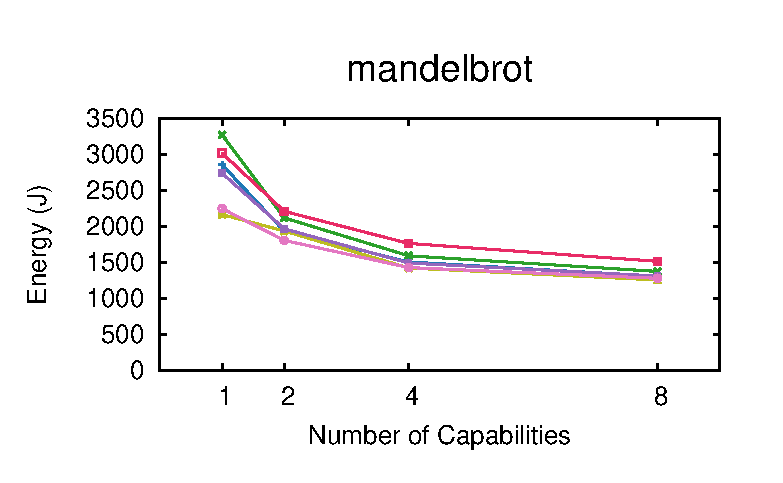
\includegraphics[width=0.47\linewidth]{images/conc_bench/mandelbrot-i7-energy} &
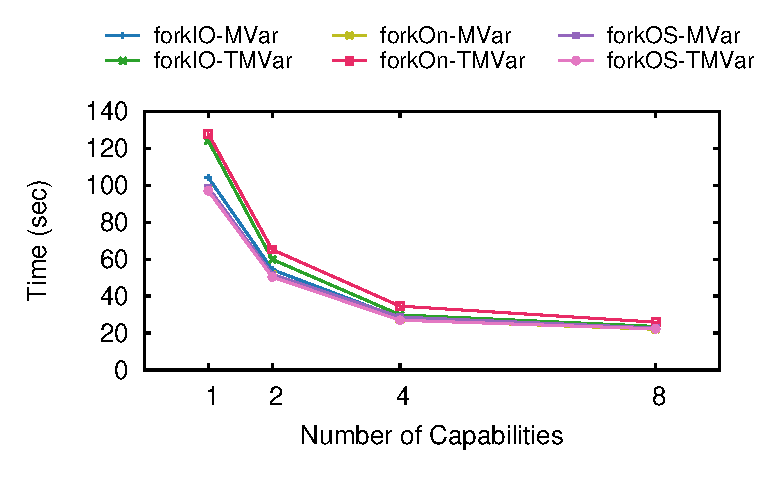
\includegraphics[width=0.47\linewidth]{images/conc_bench/mandelbrot-i7-time} \end{array}
$
\footnotesize{Source: Made by the author.}
\label{fig:other-machine-conc}
\end{figure}

It is also not possible to generalize the results to other versions of GHC. Changes in the runtime system, for example, can lead to different results. This work also did not explore the influence of the various compiler and runtime settings of GHC. As the options range from GC algorithms to scheduling behaviour, it can have a significant impact on performance, especially for concurrency. For the benchmarks we developed, we used the default settings of GHC. For the ones from CLBG, we used the same settings used there to preserve the performance characteristics intended by the developers.

One further threat is related to our measurement approach We have employed RAPL to measure energy consumption. Thus, the results could be different for external measurement equipment. Nonetheless, previous work~\citep{hahnel:2012} has compared the accuracy of RAPL with that of an external energy monitor and the results are consistent.

\chapter{A Guideline for Developers}
\lipsum[1-1]


\section{Use \forkOn for embarrassingly parallel problems}
\sstate{Description:} Both the performance and energy consumption of a program can be improved by using \forkOn to create new threads of execution when there is little or no dependency among these threads and they perform almost the same amount of work.
\newline

\sstate{Rationale:} A problem that can be decomposed into parallel tasks that do not need to communicate with each other to make progress is called \emph{embarrassingly parallel}~\cite{herlihy:2012}. Three of the benchmarks from \chapref{chp:study} fits this description: \mandelbrot, \regex and \spectral. The results from our study has shown that, for these benchamrks, the variants using \forkOn superseded the others in both performance and energy consumption. This result shows that manually distributing the workload in an even manner among the capabilities instead of handing this job to the runtime system scheduler improves performance. It makes sense because we know before hand that each worker thread is doing exactly the same amount of work. In such scenarios, there is no need for migrating a thread from one capability to another since an even distribution is the one which contributes the most for the program's progress. It makes sure that each capability will have the same workload. So using \forkOn in these cases reduces the overhead incurred by the Haskell runtime system.

\begin{figure*}[tp]
\caption{Performence of \mandelbrot and \spectral with different number of workers}
\centering
$
\begin{array}{ccc}
 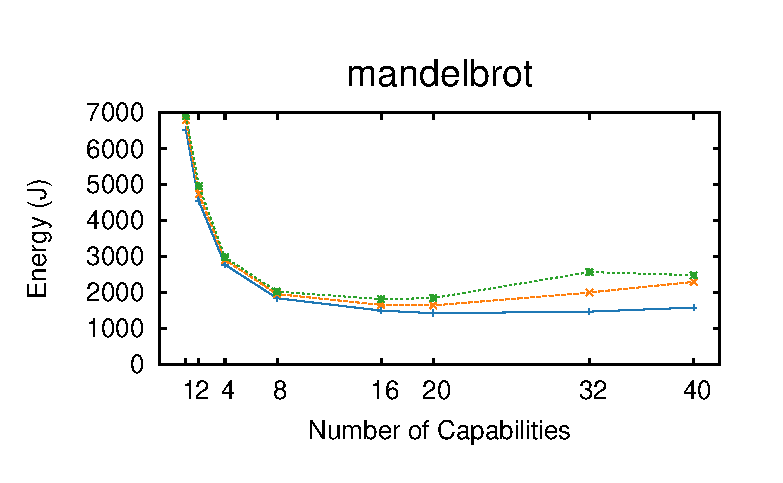
\includegraphics[width=.48\textwidth]{images/conc_bench/mandelbrot-Xt-energy} &
 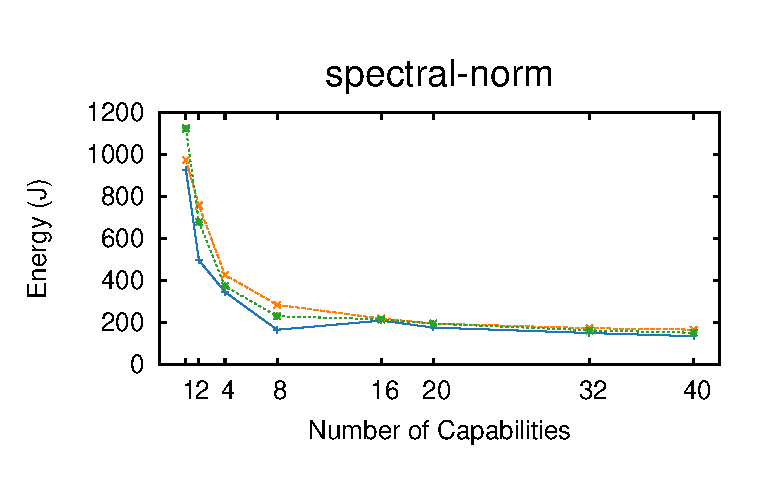
\includegraphics[width=.48\textwidth]{images/conc_bench/spectral-norm-Xt-energy} \\

 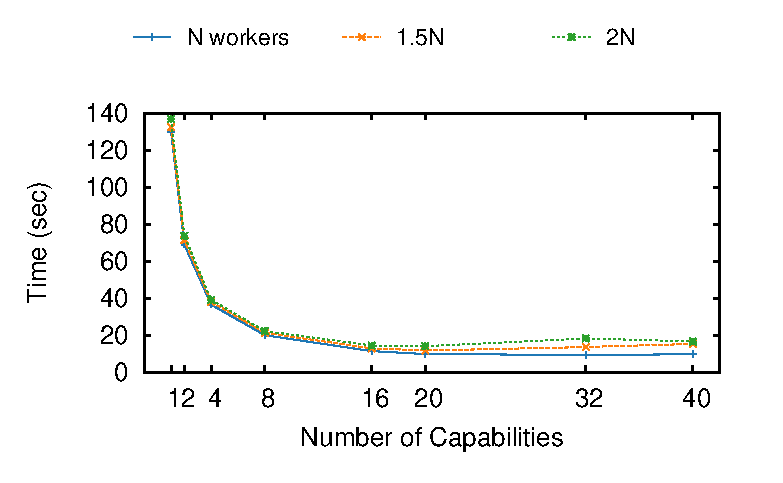
\includegraphics[width=.48\textwidth]{images/conc_bench/mandelbrot-Xt-time} &
 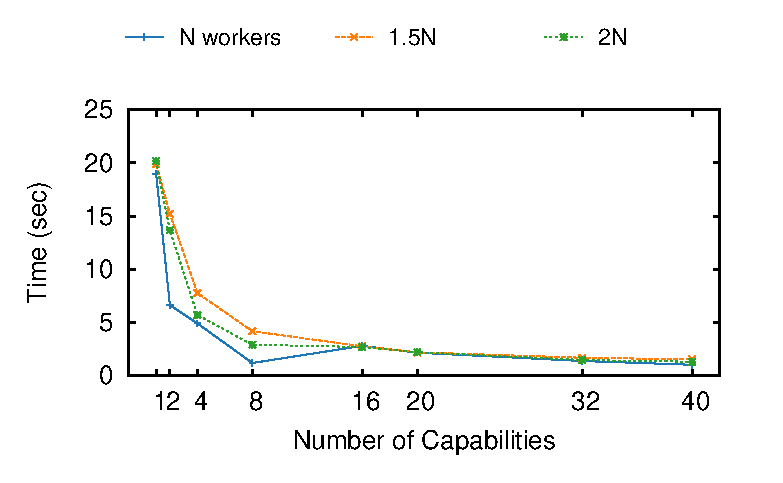
\includegraphics[width=.48\textwidth]{images/conc_bench/spectral-norm-Xt-time} \\
\end{array}
$
\footnotesize{Source: Made by the author}
\label{fig:more-threads}
\end{figure*}

However, \regex is implemented diffenrently from \mandelbrot and \spectral. The first one uses a fixed number of worker threads (350) while the others the number of threads can be set by the developer. For the experiments of \chapref{chp:study}, we set these benchmarks to spawn as many threads as the number of capabilities. We decided to run another experiment with \mandelbrot and \spectral to check how they behave if we overpopulate the capabilities' work queue. In \figref{fig:more-threads}, we can see the results for the \forkOn-\MVar variant of both benchmarks with $N$, $1.5N$ and $2N$ worker threads, where $N$ is the number of capabilities. As we can see, although the performance is similar, one thread per capability is the configuration with the best performance. This result makes sense because it reduces the costs of context-switching between threads of the capabilities' work queue. Thus, creating one worker thread per capability benefits both performance and energy consumption.

\begin{figure*}[tp]
\caption{Performence of \regex and \spectral using \texttt{-qa} and \texttt{-qm}}
\centering
$
\begin{array}{ccc}
 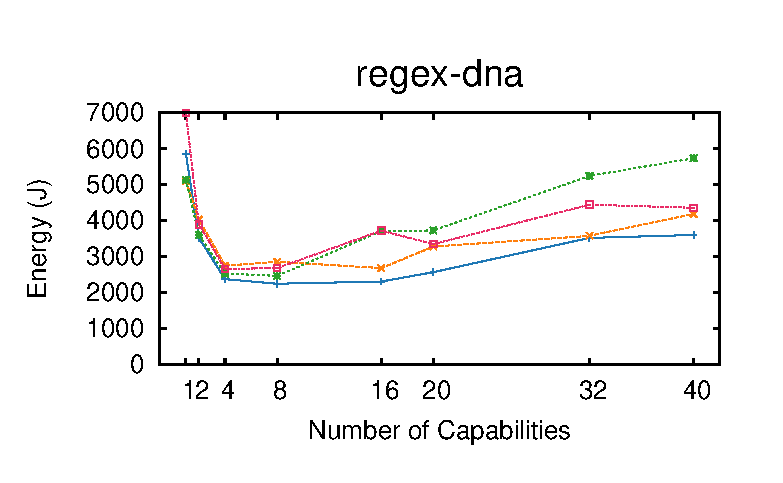
\includegraphics[width=.48\textwidth]{images/conc_bench/regex-dna-qX-energy} &
 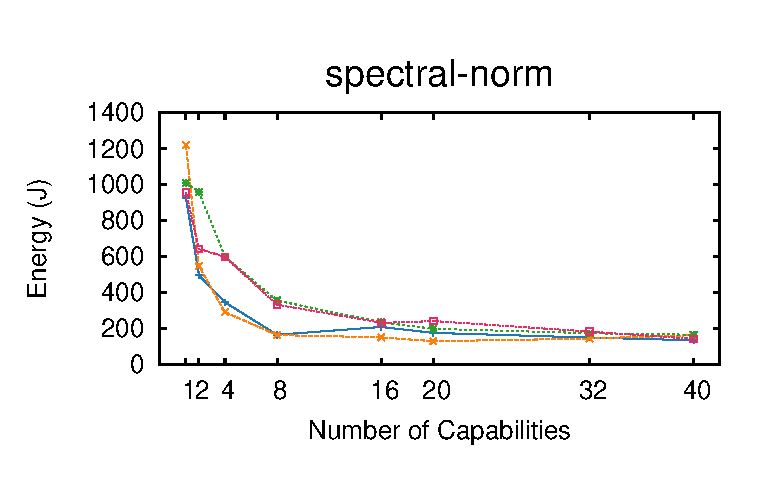
\includegraphics[width=.48\textwidth]{images/conc_bench/spectral-norm-qX-energy} \\

 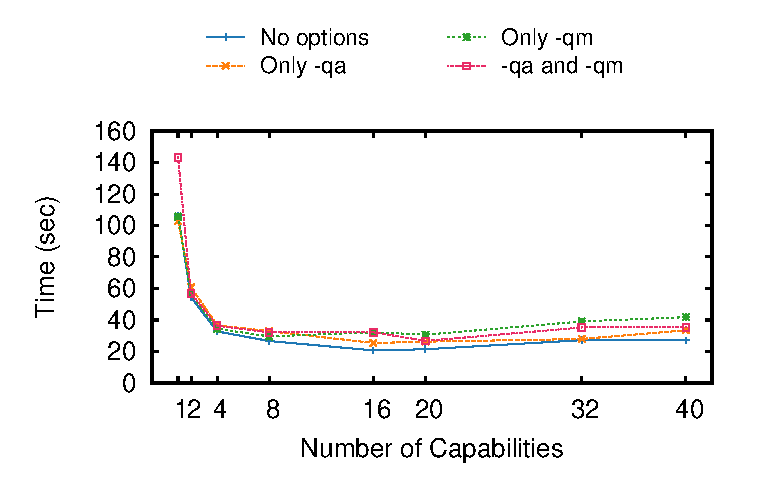
\includegraphics[width=.48\textwidth]{images/conc_bench/regex-dna-qX-time} &
 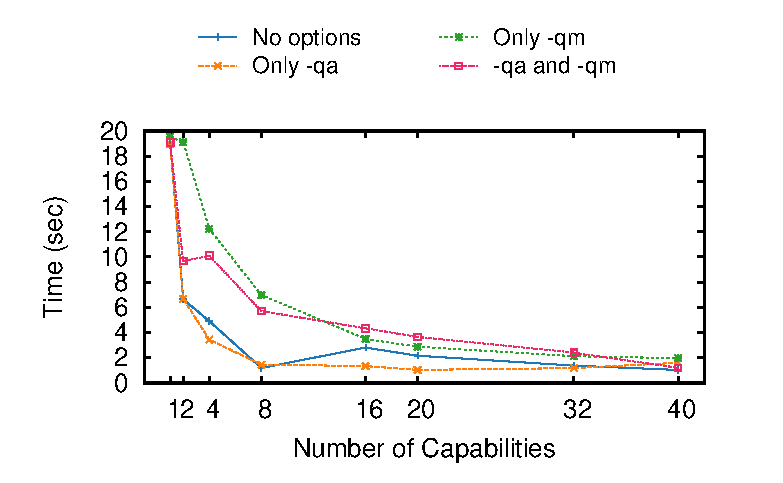
\includegraphics[width=.48\textwidth]{images/conc_bench/spectral-norm-qX-time} \\
\end{array}
$
\footnotesize{Source: Made by the author}
\label{fig:rts-flags}
\end{figure*}

Additionally, there are two \ac{rts} options that, in conjunction with \forkOn, can affect the performance of some embarrassingly parallel algorithms. The first one is the \texttt{-qa} option. It tries to pin OS threads to CPU cores using native OS facilities\footnote{In Linux, GHC uses the \texttt{sched\_setaffinity()} syscall}. Using this option, the OS threads associated with a capability \emph{i} are bound the CPU core \emph{i}. The other one is the \texttt{-qm} option. It disables automatic migration of threads between CPUs. The former seems to fit perfectly in this context since it increases the probability of a Haskell thread being kept running on the same CPU core during the execution of the program. However, it is not clear how different the latter is from simply creating all threads with \forkOn as we are proposing here. To get a picture of their influence, we executed our embarrassingly parallel benchmarks with these options. In \figref{fig:rts-flags} we show results for the \forkOn-\MVar variant of both \regex and \spectral. Here, we executed the benchmarks without either of the options, only with \texttt{-qa}, only with \texttt{-qm}, and with both options. As we can see, the \ac{rts} options affect the performance of both benchmarks. However, the behavior is not predictable. In \spectral, using only \texttt{-qa} improves both performance and energy consumption regardless of the number of capabilities. In \regex, however, using any combination of the \ac{rts} options has a negative impact on performance. It also increases considerably the energy consumption for more than eight capabilities. We recommend developers to experiment with these options to assess how they affect the performance of a given program.

\section{Avoid setting more capabilities than available CPUs}
\sstate{Description:} Using more capabilities than the number of available virtual CPU cores can seriously degrade both performance and energy consumption of a concurrent Haskell program.
\newline

\sstate{Rationale:} A capability is thought to act as an abstraction of a CPU for the Haskell runtime system. It is the entity that can execute Haskell code. This definition implies that we can achieve maximum parallelization by creating as many capabilities as the number of CPUs. In fact, this is precisely what the official \ac{ghc} documentation recommends for developers: to set \texttt{N} to be the same as the number of the processor's CPU cores. In our experiments from \chapref{chp:study}, we analyzed how each benchmark behaved for different capabilities settings. The results have shown that, for most benchmarks, the performance improved as we added more capabilities. It also confirmed the intuition that it does not make sense to outnumber the CPU cores. For eight of our benchmarks, both the performance and energy consumption were severely impaired by going from \texttt{N=40} to \texttt{N=64}.

However, modern Intel processors are equipped with a feature called \emph{hyperthreading}. This technology increases the number of independent instructions in the processor's pipeline. For each processor core that is physically present, the operating system addresses two separate virtual cores. So from the developer's point of view, there is twice the number of CPU cores available. In this context, the \ac{ghc} documentation leaves as an open question if virtual cores should be accounted: \emph{"Whether hyperthreading cores should be counted or not is an open question; please feel free to experiment and let us know what results you find."}\footnote{\url{http://downloads.haskell.org/~ghc/7.10.2/docs/html/users\_guide/using-smp.html\#ftn.idp12916656}}. In our experiments, only one benchmark presented a significant improvement in both performance and energy consumption when going from \texttt{N=20} to \texttt{N=40}. All the others were negatively impacted by this change, which suggests that, in general, virtual cores should not be accounted for setting the number of capabilities.


\section{Avoid using \forkOS to spawn new threads}
\sstate{Description:} Using \forkOS undeliberately to spawn new threads of execution can degrade both performance and energy consumption of a concurrent Haskell program.
\newline

\sstate{Rationale:} [[ TODO ]]

\chapter{Related Work}

\section{Refactoring}
\lipsum[1-3]


\section{Performance Analysis in Haskell}
\lipsum[1-3]


\section{Software Energy Consumption}
\lipsum[1-3]

\chapter{Conclusion}

\section{Contributions}
\lipsum[1-4]


\section{Future Work}
\lipsum[2-4]


\begin{references}
  \bibliography{references}
\end{references}

\theappendix
\chapter{The \spectral Benchmark}\label{ap:benchmark}

This benchmark is part of \acl{clbg} suite. It is based on a MathWorld challenge called \emph{"Hundred-Dollar, Hundred-Digit Challenge Problems"} by Eric W. Weisstein\footnote{http://mathworld.wolfram.com/Hundred-DollarHundred-DigitChallengeProblems.html}. To submit a solution for this problem on \acl{clbg}, the program should not only give the correct result, but also use the same algorithm to calculate that result. Each program should:

\begin{enumerate}
  \item Calculate the spectral norm of an infinite matrix A, with entries $a_{11}=1, a_{12}=\frac{1}{2}, a_{21}=\frac{1}{3}, a_{13}=\frac{1}{4}, a_{22}=\frac{1}{5}, a_{31}=\frac{1}{6}...$
  \item Implement 4 separate functions to:
  \begin{itemize}
    \item Return element $(i,j)$ of infinite matrix $A$
    \item Multiply vector $V$ by matrix $A$
    \item Multiply vector $V$ by matrix $A$ transposed
    \item Multiply vector $V$ by matrix $A$ and then by matrix $A$ transposed
  \end{itemize}
\end{enumerate}

Following, we show the implementation we used for this benchmark. In this case, we are showing only the  source code for the \forkIO variant as the refactoring to change the thread management construct is straightforward. We split it in multiple sections to better present it here, but it can be seen as a whole on GitHub\footnote{https://github.com/green-haskell/concurrency-benchmark}. \autoref{code:b_criterion} is the entry point of the program where we define the Criterion benchmark that will call \spectral. \autoref{code:b_main} and \autoref{code:b_eign} are common parts that were not refactored. \autoref{code:b_mvar}, \autoref{code:b_tmvar} and \autoref{code:b_tvar} show the implementation of the \texttt{CyclicBarrier} type for the \MVar, \TMVar and \TVar variants, respectively. Finally, \autoref{code:b_functions} shows the fours functions required by the problem statement.

\begin{listing}
  \caption{The Criterion benchmark}
  \inputminted[fontsize=\scriptsize]{haskell}{appendix/a-0.tex}
  \label{code:b_criterion}
\end{listing}

\begin{listing}
  \caption{Entry point of \spectral}
  \inputminted[fontsize=\scriptsize]{haskell}{appendix/a-1.tex}
  \label{code:b_main}
\end{listing}

\begin{listing}
  \caption{A function to calculate the eigenvalue of a matrix}
  \inputminted[fontsize=\scriptsize]{haskell}{appendix/a-2.tex}
  \label{code:b_eign}
\end{listing}

\begin{listing}
  \caption{\texttt{CyclicBarrier} defined for the \MVar variant}
  \inputminted[fontsize=\scriptsize]{haskell}{appendix/a-3.0.tex}
  \label{code:b_mvar}
\end{listing}

\begin{listing}
  \caption{\texttt{CyclicBarrier} defined for the \TMVar variant}
  \inputminted[fontsize=\scriptsize]{haskell}{appendix/a-3.1.tex}
  \label{code:b_tmvar}
\end{listing}

\begin{listing}
  \caption{\texttt{CyclicBarrier} defined for the \TVar variant}
  \inputminted[fontsize=\scriptsize]{haskell}{appendix/a-3.2.tex}
  \label{code:b_tvar}
\end{listing}

\begin{listing}
  \caption{The four functions to manipulate the matrix}
  \inputminted[fontsize=\scriptsize]{haskell}{appendix/a-4.tex}
  \label{code:b_functions}
\end{listing}


\end{document}
